\documentclass{memoir}

%\usepackage{fancyhdr}
\usepackage{xcolor}
\usepackage{hyperref}
\usepackage{graphicx}
\usepackage{enumitem}
\usepackage{verbatim}
\usepackage{framed}
\usepackage[T1]{fontenc}

\setlength{\parindent}{0pt}
\nonzeroparskip


\graphicspath{{../figures/}}
\hypersetup{
  colorlinks,
  linkcolor={red!50!black},
  citecolor={blue!50!black},
  urlcolor={blue!80!black}
}
\urlstyle{same}
\setlength{\headheight}{15.2pt}
\pagestyle{simple}
%\fancyhf{}
%\lfoot[$\the\numexpr\value{page}$]{} %-1 to take into account title page.
%\rfoot[]{$\the\numexpr\value{page}$}

\begin{document}

\begin{titlingpage}
  
  \centering
  \vspace{0.5 cm} 
  \vbox{\hrule width \hsize \kern 1mm \hrule width \hsize height 2pt}
  \vspace{0.4cm}
  \textsc{\LARGE The Linkage Coder program User Manual} \\[2.0 cm]
% \vspace{0.4 cm}
 %\rule{\linewidth}{0.4 mm} \\
 %\vspace{1.0 cm}
 \vfill 
 \begin{minipage}{0.4\textwidth}
   \begin{center}
     \emph{Wouter Spekkink}
   \end{center}
   \begin{center} \large
     \textsc{\today} \\[10.0 cm]
   \end{center}
 \end{minipage}~
\end{titlingpage}

\tableofcontents
\chapter{Introduction}
\label{chap:introduction}

\section{The Linkage Coder program}
\label{sec:eventcoderprogram}

The document you are currently reading is the user manual for the open source (GPL 3.0) software tool called \emph{\textbf{Event Coder}}, written by me (Wouter Spekkink) in C++ and Qt5 \footnote{The source code is available from my Github page (see chapter \ref{chap:contactdetails}).}.

The program is intended to facilitate in the qualitative coding of event data. In this case, event data refers specifically to bracketed, chronologically ordered, qualitative data that captures activity that occurred in some type of process. My thinking about what event data is, and much of the terminology that I use, is heavily inspired by activities carried out as part of the Minnesota Innovation Research Program\footnote{see especially Poole, M. S., Van De Ven, A. H., Dooley, K., \& Holmes, M. E. (2000). \emph{Organizational Change and Innovation Processes: Theory and Methods for Research.} Oxford: Oxford University Press. I was not involved in this work in any way.}. I have many other sources of inspiration that I will not mention in this manual. It should be easy enough to find my other sources of inspiration in the publications I have written (see my contact details in chapter \ref{chap:contactdetails}).

Why is it useful to have this tool? Over the past years I have worked together with other people (especially Frank Boons) to develop and use various methods and tools for the study of social processes. In doing so, we have always worked with the principle that our fundamental units of analysis should be events, that is, things that ``happened'' or ``came to pass'', as opposed to, for example, variables. Based on ideas developed by the researchers from the Minnesota Innovation Research Program, we started collecting data in the form of \emph{incidents}, which are qualitative, bracketed descriptions of activity, which consist (at least) of (1) an indication of the time at which the activity occurred, (2) a (brief) qualitative description of the activity, and (3) the source of data (e.g., a document, an interview, personal conversation)\footnote{The descriptions (point 2) are typically created by the researcher him/herself. When I am using textual sources (e.g., documents, web pages, interview transcripts), I also like to add the ``raw'' text on which my incident description was based.}. During the collection of event data, we create numerous incidents, which we store in chronologically ordered event data sets.

Again, following ideas developed by researchers from the Minnesota Innovation Research Program, we have been using qualitative coding procedures as a step in the analysis of event data. There can be multiple purposes for doing this, but at least one important purpose is (roughly) to relate the \emph{empirical observations} recorded in incidents to \emph{theoretical constructs}, which are not directly observable and  play a role in \emph{theories} that are developed to explain the \emph{empirical phenomenon} of interest to us. The \textbf{\emph{Event Coder}} program can be used to facilitate such qualitative coding procedures. The program allows the user to assign attributes to incidents to express how these incidents relate to theoretically relevant constructs. In addition, it also allows one to assign relationships to incidents to express what \emph{relationships} between what \emph{entities} are indicated by the observed incidents, which can be useful in studies that aim to answer questions about \emph{process} and \emph{structure} and/or relationships between the two for different ways in which one could go about this). I and others have done some of these things using simpler tools, such as assigning attributes to incidents by simply typing their labels into Excel files. However, the \textbf{\emph{Event Coder}} program makes this process more systematic and less error prone, and therefore (I hope) less painful.

This manual gives an in-depth introduction to the program and its functionality. In the remainder of the introduction, I offer some additional background to the program, and I introduce some necessary disclaimers. Consider reading these disclaimers before you send me angry emails. In chapter \ref{chap:preparations} I go into some of the assumptions that the program builds on (e.g., about the data sets that you will code), and what preparations (i.e., things you are assumed to have done before using the program) this implies. In chapter \ref{chap:usingtheprogram} I go through some of the basic features of the program that do not involve qualitative coding itself, such as importing data, and saving and loading files. In chapter \ref{chap:usingtheprogram2} I explain the coding features of the program. I conclude the main body of the manual with chapter \ref{chap:whatisnext}, discussing some of the things that one could do with the data that the program exports. My contact details can be found in chapter \ref{chap:contactdetails}. 

\section{Part of a bigger program}
\label{sec:partofbiggerprogram}

It is very important for the reader to realise that, even though I wrote the \textbf{\emph{Event Coder}} as a standalone program, I wrote it primarily with the intention to later integrate it, as a module, in a larger program. The idea is that, in the larger program, you would be able to do everything from entering data into your data set, coding the data in various ways, doing basic forms of analysis, creating visualisations, and exporting data files that can be easily imported into other useful software. The current (standalone) version of the program still requires you to (1) create your data set with external spreadsheet software (e.g., LibreOffice Calc or Excel), (2) use external software to further visualise and analyse the coded data.

\textbf{And here is a very important thing to consider before you start using the current version of the program:} I would advice you to at least skim through chapter \ref{chap:whatisnext} first. In this chapter, I offer some examples of how the data that the program exports can be imported into other software, and what possibilities this offers. Making use of this program probably only makes sense if these possibilities are actually interesting for your work.

Please, also see section \ref{sec:exportingdata} to get a good idea of what kind of data the program actually exports. The motivations for the choices that I made in this are perhaps not immediately obvious to everyone, and probably for some they will not become obvious until I actually get to integrating my work in the larger program that I have in mind. However, one thing I can say is that I have a strong preference for storing, visualising, and analysing event data (and related data) in some type of graph format. This can be achieved most efficiently if data are eventually stored either as \textbf{nodes}, \textbf{relationships between those nodes}, or \textbf{properties of nodes or relationships}. This is the reason why the data that the program exports take the form of (primarily) node lists and edge lists, which would allow you to import and visualise the data into various software tools for network visualisation \footnote{see, for example, \url{https://gephi.org}, which is my favourite.}.  

\section{Other disclaimers}
\label{sec:disclaimers}

Throughout the introduction, I already snuck in a few disclaimers, such as the fact that my work on this particular (standalone) version of the program will probably stop once I get to integrating it as a module into a larger program. There are several additional disclaimers I would like to make here. 

It is very important that the user realises that I wrote this program, in the first place, for personal use, and that I only make it available for free in case other people may find it helpful in their work. However, you will use the program at your own risk. I do \textbf{not} take any responsibility for problems that you run into when using the program. That being said, I am always open to receiving comments, positive or negative, about problems that may occur, bugs you encounter, features you would like to be included, and so on. If you do indeed run into problems as a result of using this program, I am willing to help you think of a solution. You can find my contact details in chapter \ref{chap:contactdetails} of this manual.

The user should also realise that I am \textbf{not} a professional programmer. With some help from the Internet, I taught myself how to code to keep my mind occupied during some of the lonely evening hours I spent in a campus apartment somewhere in Shenyang. I never had any formal training in writing code, and I probably make a lot of ugly mistakes, write inefficient code, and overlook simple solutions for the various problems I face while writing code. While I always try to improve my coding skills, this requires a lot of time, energy, and verbal abuse of my computers\footnote{If you happen to be someone with more experience in writing code, feel free to go to my Github page (see chapter \ref{chap:contactdetails}) to inspect the source code of this program, and if you have the time and patience, please offer me suggestions on how to improve my skills.}. This means that I will not always have the time, energy and/or the skills required to fix certain bugs, add new features, and etcetera.

I also do \textbf{not} have a team of beta-testers to help me test the program. You are basically it. Congratulations! If I had T-shirts, I would ship you one to give you some recognition, but unfortunately I have no budget for that. The program is still fairly simple in structure, and I tried to get rid of most bugs by doing my own testing. However, the program is already complex enough for me to overlook things, so there is a good possibility to several annoying bugs remain. The only way to find these, sadly, is to encounter them while using the program. Fortunately for you, if there is one thing that I really hate, it is having bugs in my programs. If you do encounter a bug, please contact me (see chapter \ref{chap:contactdetails}) ASAP, and I (or we) will try to figure out what is wrong, so that I can fix it.



\chapter{Preparations}
\label{chap:preparations}

\section{It is all about the data}
\label{sec:allaboutdata}


As mentioned in section \ref{sec:partofbiggerprogram}, the \textbf{\emph{Event Coder}} program is designed to be eventually integrated into a larger program. In that larger program, data would be entered into, and managed by the program directly. For now, however, the \textbf{\emph{Event Coder}} program needs to import all data from external sources, that is, files created by the user before using the program. The program can be understood to make some assumptions about the nature of these files, and if these assumptions are not met while reading files, the program may not work as it should.

Fortunately, creating files that can be read by the program is not difficult. Moreover, the ways these files should be created follow logically from the kind of research approach that this program is designed to fit into. In this chapter, I go into all things that the user should think of well before using this program, preferably in the stage before data collection. Most of these details have to do with the kind of data sets that the program ``expects'' you to work with.

\section{Data sets}
\label{sec:datasets}

The program expects that you will import data from what I will call an \emph{event data set}, which is nothing more then a table of chronologically ordered \emph{incidents}. The idea of having such data sets, and the concept of incidents are both based on ideas developed during the Minnesota Innovation Research Program\footnote{see especially Poole, M. S., Van De Ven, A. H., Dooley, K., \& Holmes, M. E. (2000). \emph{Organizational Change and Innovation Processes: Theory and Methods for Research.} Oxford: Oxford University Press. I was not involved in this work in any way.}. An incident is a bracketed, qualitative description of an observed activity, which includes, at least, the following information:
\begin{enumerate}
\item{An indication of the time at which the incident occurred.}
\item{A brief (qualitative) description of the activity, including a description of the actors/entities responsible for the activity.}
\item{A reference to the source of data.}
\end{enumerate}

This is still a very open description of what an incident actually can contain. As a social scientist, I am typically mostly interested in \emph{human activity}, that is, in activity performed by human beings. That, in itself, is still a very broad category, and it leaves open the question at what level of abstraction that activity can and/or should be described\footnote{One of my other sources of inspiration is the work of Peter Abell on Comparative Narratives. Abell's work engages more or less directly with questions of how to describe activity at different levels of abstraction. See especially: Abell, P. (1987). \emph{The syntax of social life: the theory and method of comparative narratives}. Oxford, Angleterre: Clarendon.}. We may also understand the concept of activity in a much broader sense, such that we also include natural occurrences, such as volcanic eruptions, an apple that falls from a tree, or the wind that blows. In the end, what makes sense to count as activity will depend on your research questions, your theoretical orientation, and probably on who you count among your favourite philosophers.

Fortunately, the \emph{\textbf{Linkage Coder}} program does not care about your definition of activity. However, whatever definition you decide to work with, the program does care about how exactly you store information on that activity as incidents in your data sets. In the type of event data sets that we work with here, the very first row of data is always the \textbf{header} of the file, which contains the names of the columns in the data file (see figure \ref{fig:datasetstructure}). All the remaining rows of the data set represent individual incidents. The three aspects of incidents that we mentioned above (timing, description and source) should be stored in separate columns. You may label and position these columns however you like, but we expect these columns to be there.

\begin{figure}[h!]
  \centering
  \caption{The expected structure of event data sets.}
  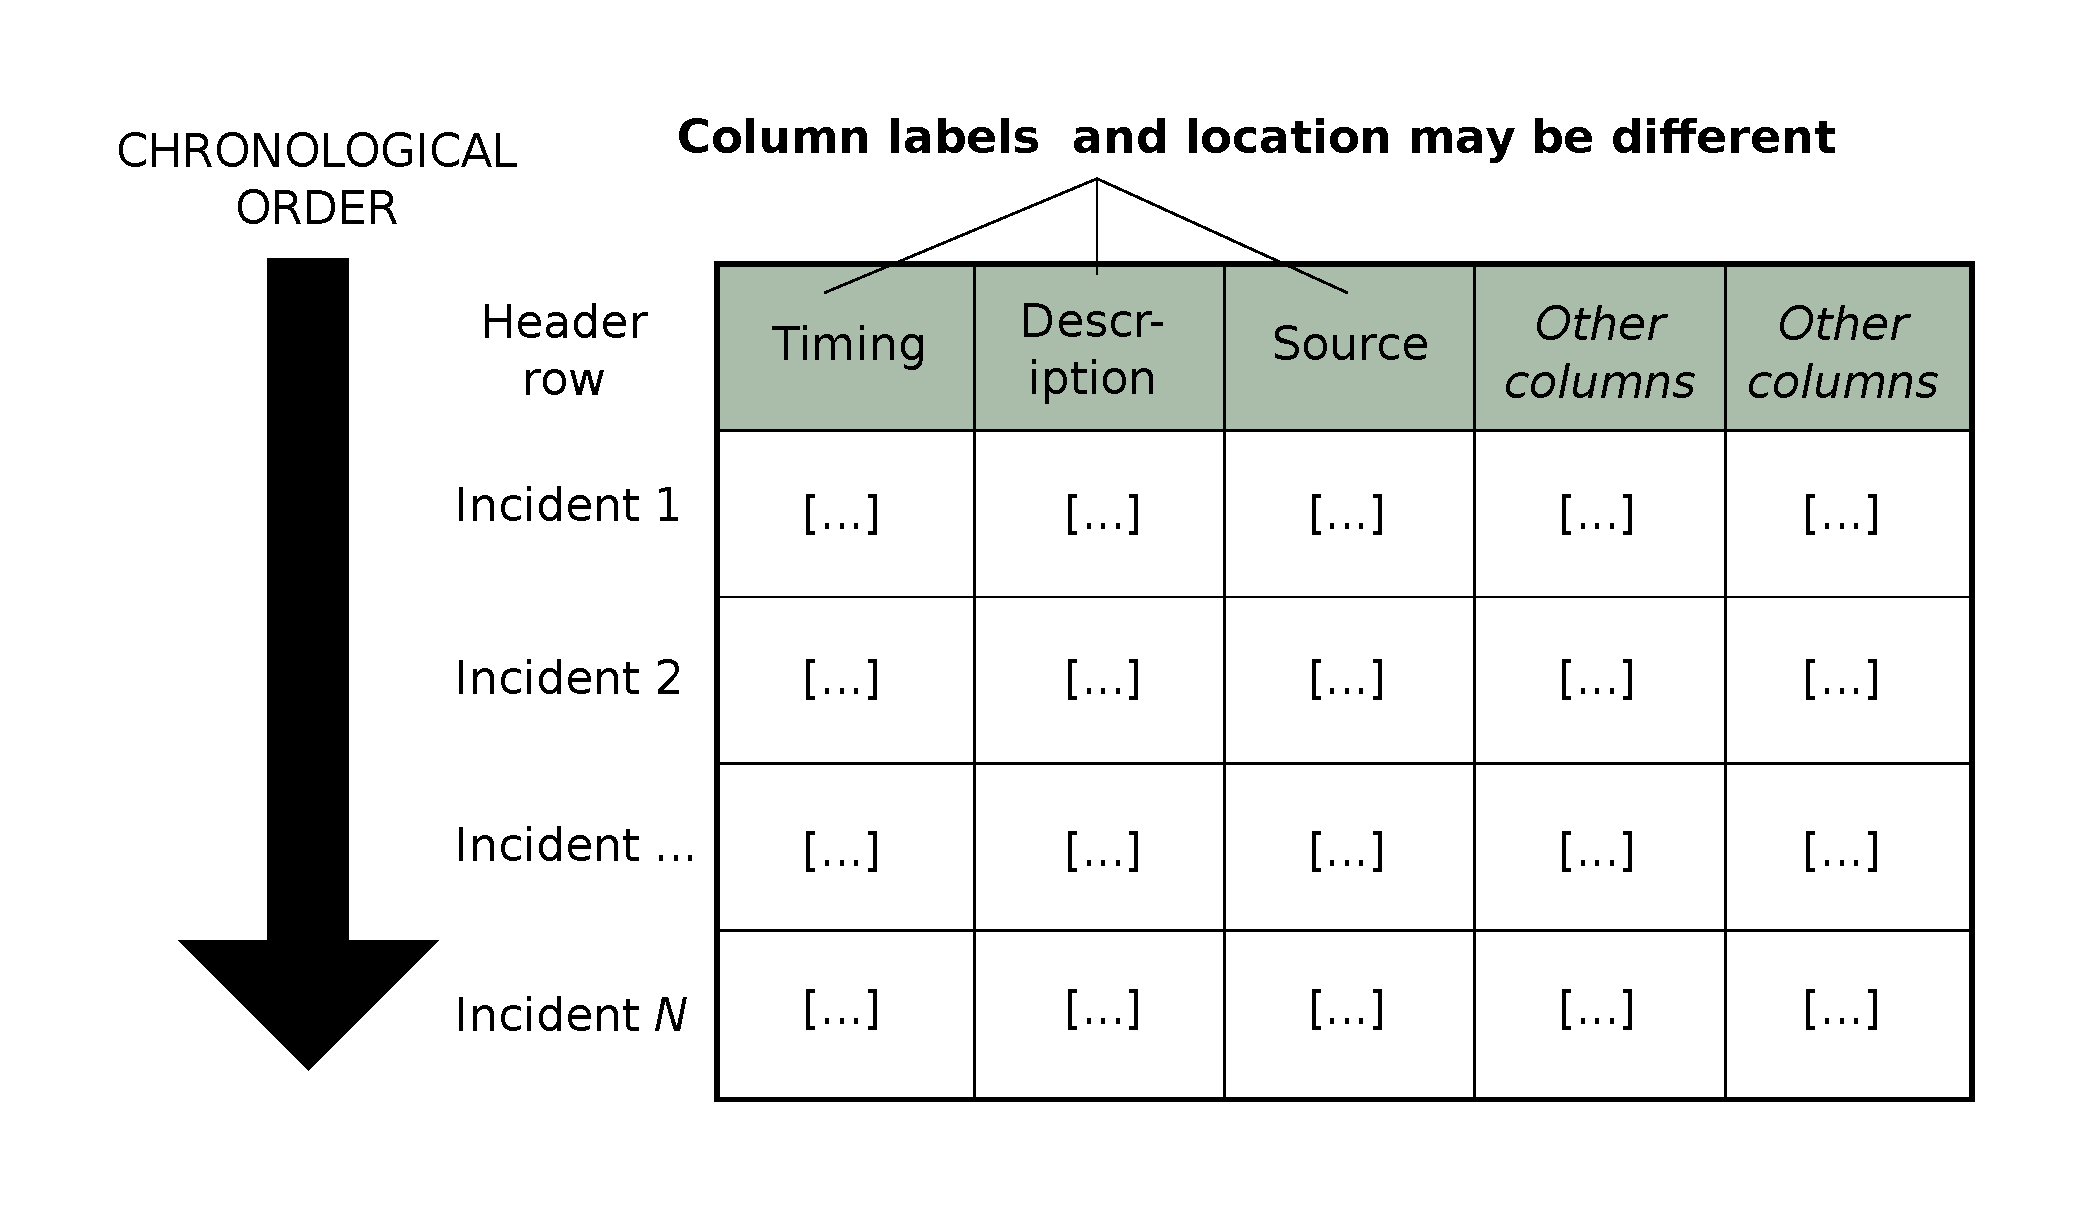
\includegraphics[width=100mm]{Diagram_4.pdf}
  \label{fig:datasetstructure}
\end{figure}

You may also add additional columns to your data set, to expand on the information about incidents that the data set records. For example, I made a habit of also including fragments of text from the original sources of data on which I based my incident descriptions. In my opinion, this makes the process of coding incidents both easier, and more transparent.    

Another important assumption that the \textbf{\emph{Linkage Coder}} program makes about your data set is that it is chronologically ordered. That means that the incident reported in a given row is assumed to have happened after the incident preceding it (of course, with the exception of the first incident in the data set). Even if two or more incidents actually happened simultaneously, based on their position in the data set, the program will always assume that there is an order in their occurrence. In practice, this should not be a serious problem.

These are basically all the assumptions that the program makes about the overall structure of your data set. However, there are some other practical considerations to be taken into account. The most important one is that the \textbf{\emph{Linkage Coder}} program can only import data from so-called \emph{comma-delimited files} (I will refer to them as csv files), which can be recognised by their ``*.csv'' extension (e.g., ``My\textunderscore Dataset.csv''). These files are very much like plain text files (``*.txt''), but they use so-called \emph{delimiters} (most often commas or semicolons) to distinguish between different columns. You can open csv files in a basic text editor to see what this looks like (see figure \ref{fig:csvfile}).

\begin{figure}[h!]
  \centering
  \caption{What a csv file looks like in a basic text editor.}
  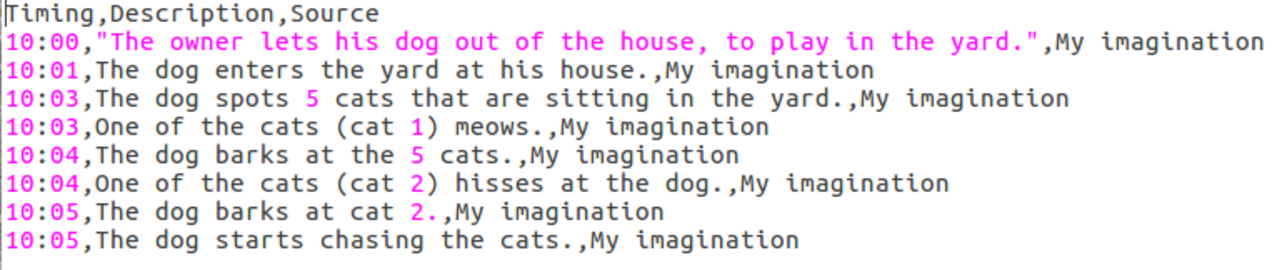
\includegraphics[width=80mm]{Screenshot_19.pdf}
  \label{fig:csvfile}
\end{figure}

Spreadsheet software, like Excel or LibreOffice Calc, typically allows you to store tables as csv files, using the \textbf{``Save As''} option\footnote{I have encountered a few people who misunderstood how this works, and who simply tried to convert files by changing their extension. For example, they would rename a file called ``My\textunderscore Dataset.xls'' to ``My\textunderscore Dataset.csv''. This will not work, because it will not actually change the file itself. It is more likely that you will just render your file unreadable for most software, because the software will think it is reading a csv file, while it is really reading an xls file that is only disguised as a csv file.}. Some software, like Excel, will use a delimiter that is set ``system-wide''. If you are unsure what delimiter your system uses, just open your csv file with a text editor, and see what characters are used to separate columns. You will need to know what delimiter your files use to be able to import them properly. Other software, like LibreOffice Calc, allows you to choose what delimiter to use when you save the csv file.

So, you can create your data set using in any spreadsheet software that you prefer. You can also store your data set in any format that you prefer while building it. The important thing is that you should be able to store it as a simple csv file as soon as your are ready to import it into the \textbf{\emph{Linkage Coder}} program. For example, while working on my data sets, I typically store my data in ods files or xls files, but as soon as I want to start coding my data, I will use the \textbf{``Save as''} feature of whatever program I am working with to store a csv file.   

\subsection{Other notes}
\label{sec:othernotesdatasets}

There is a little bit more going on in csv files than what is shown in a regular text editor. What figure \ref{fig:csvfile} does not show, for example, is that there are also hidden characters present in the file that tell the computer where each line of data ends (so-called newline symbols: \textbackslash n). You usually do not have to worry about the presence of such characters, with some small exceptions. 

The \emph{\textbf{Linkage Coder}} program is not able to read csv files that have so-called newline symbols (\textbackslash n) or carriage return symbols (\textbackslash r) \emph{within} their text cells. The reason for this is that the program uses a relatively simple csv file parser, which will think that a new line of data will start after encountering one of these symbols (each line of data in a csv file will end with a newline symbol by default). Fortunately, inserting such symbols into the text cells will only happen if you deliberately create them, or accidentally paste them into your file. 

The program is typically able to recognise when an 'illegal' newline is encountered, and it will throw an error (see figure \ref{fig:importerror}). Solving the error is left to the user. The problem can be solved by removing all newline symbols and carriage return symbols from the csv file. These symbols are not visible in programs like Excel or LibreOffice Calc, and in both programs you will need to use special search and replace options to get rid of the unwanted symbols. I advise you to Google for ``Find and replace regular expressions with [your spreadsheet program]''. 

\chapter{Using the program: Basic features}
\label{chap:usingtheprogram}

\section{Loading a new dataset}
\label{sec:loadingnewdataset}

Assuming that you have a data set ready, importing the data into the program works as follows. You first need to select the csv file containing your data. For this you will click the \textbf{Select File} button (see figure %\ref{fig:importoptions}), which will open a file dialog that you can use to navigate to, and select the file.

Once a file has been selected, you will need to select the delimiter symbol that is used in the csv file to distinguish between different columns of the data table. For this, you can use the dropdown menu that reads \textbf{-Select delimiter-} by default. Four different symbols are allowed as delimiter, which are the comma (,), the semicolon (;), the colon (:), and the vertical bar (\textbar). Make sure that the delimiter that you select matches the one used in the file.

Once you have selected a delimiter, you can import the data, using the \textbf{Import data} button. Once you click this button, the program will attempt to read data from selected file and, if successful, enable all other options of the program, allowing you to start coding.   

% \begin{figure}[h!]
%   \centering
%   \caption{Options to import data.}
%   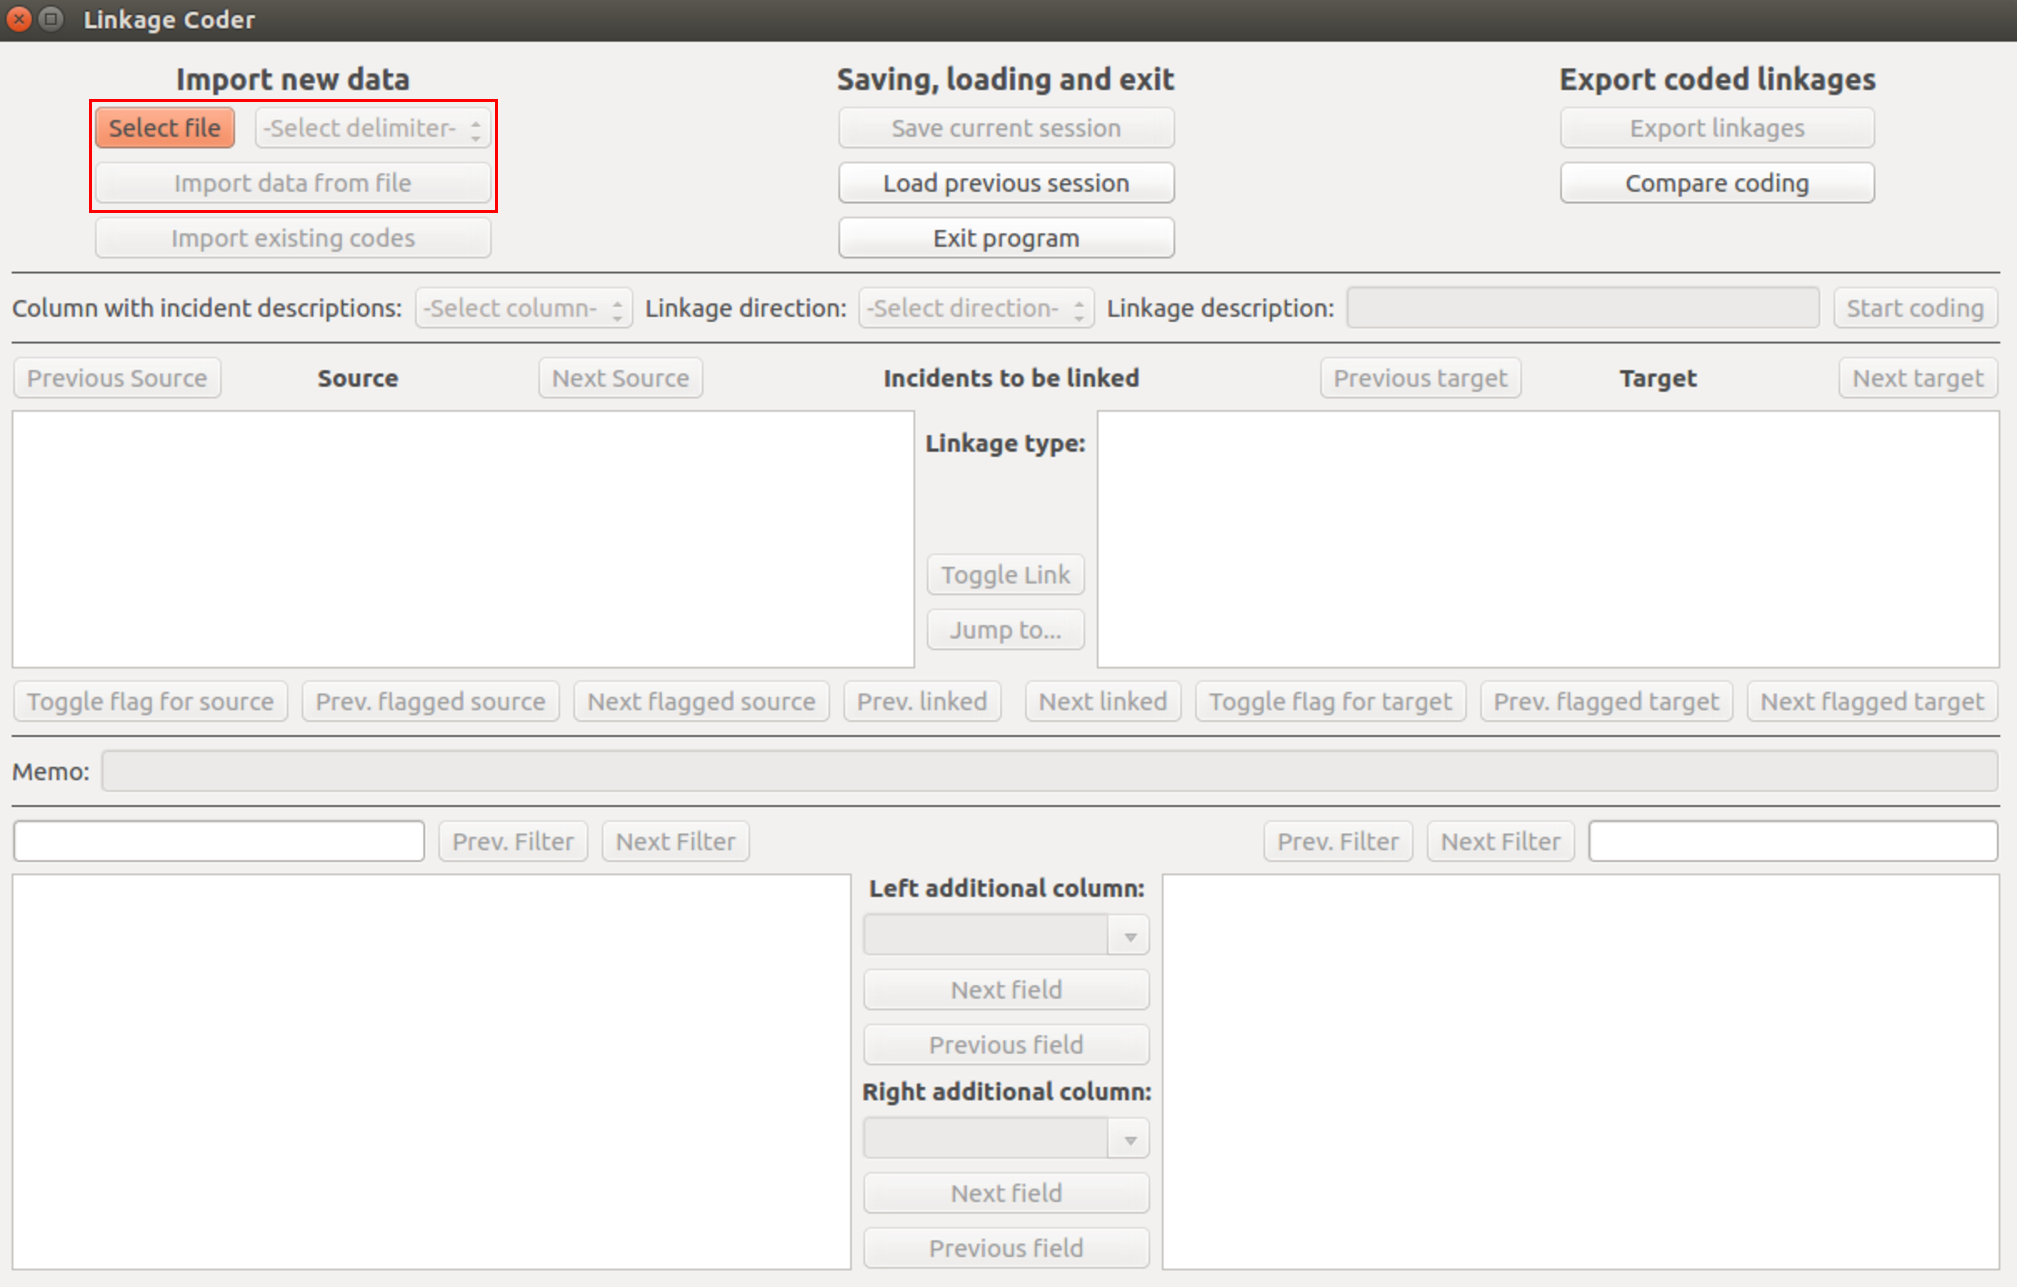
\includegraphics[width=100mm]{Screenshot_0.pdf}
%   \label{fig:importoptions}
% \end{figure}

\subsection{Problems when importing data}
\label{sec:importerrors}

If you (1) selected a valid csv file, (2) selected the correct delimiter for this file, and (3) structured your data set using instructions offered in section \ref{sec:datasets}, you should encounter no problems when importing the data. If something goes wrong when importing data, then the problem will usually lie with one of these three points.

One possibility is that you have not selected a valid csv file. I have encountered a few people that have tried to create csv files from (for example) xls-files by simply changing the file extension. Doing this will not actually create a valid csv file that can be read by the program. The correct way for creating csv files is to use the \textbf{Save as} option in your spreadsheet editor, and select to save the file with the \textbf{*.csv} extension.

If you selected the wrong delimiter, the program will usually import the data, but it will fail to distinguish between different columns of the data set, and possibly assume that the entire dataset only contains one column. This should be obvious from the texts displayed by the program. In this case, simply import the data again, using the correct delimiter. 

If you see the error message displayed in figure \ref{fig:importerror}, this means that some cells of your data set probably contain newline symbols and/or carriage return symbols that need to be removed before importing data (see section \ref{sec:othernotesdatasets}).

\begin{figure}[h!]
  \centering
  \caption{Data import error report.}
  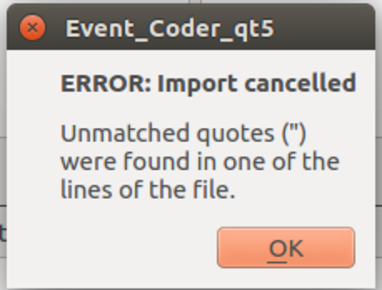
\includegraphics[width=40mm]{Screenshot_1.pdf}
  \label{fig:importerror}
\end{figure}

If you are certain that you made no mistakes in one of these points, and you still encounter problems when importing your data set, then you may have encountered a bug in the program that needs to be fixed. In that case, please get in touch with me (see chapter \ref{chap:contactdetails}).

\section{Saving and loading data}
\label{sec:savingloadingdata}

Coding a data set typically will take a long time, which is why the program allows you to save your progress, and to load the saved session at another moment. Saving data can be done by clicking the \textbf{Save current session} button (%see figure \ref{fig:saveload}). A file dialog will appear, asking you to select a location to store the file, as well as a name for the file. The files will always be saved with the ``.sav'' extension.

If you want to load a previously stored session, click the \textbf{Load previous session} button (%see figure \ref{fig:saveload}). A file dialog will appear, allowing you to navigate to, and select the file that you wish to load. 

% \begin{figure}[h!]
%   \centering
%   \caption{Saving and loading files.}
%   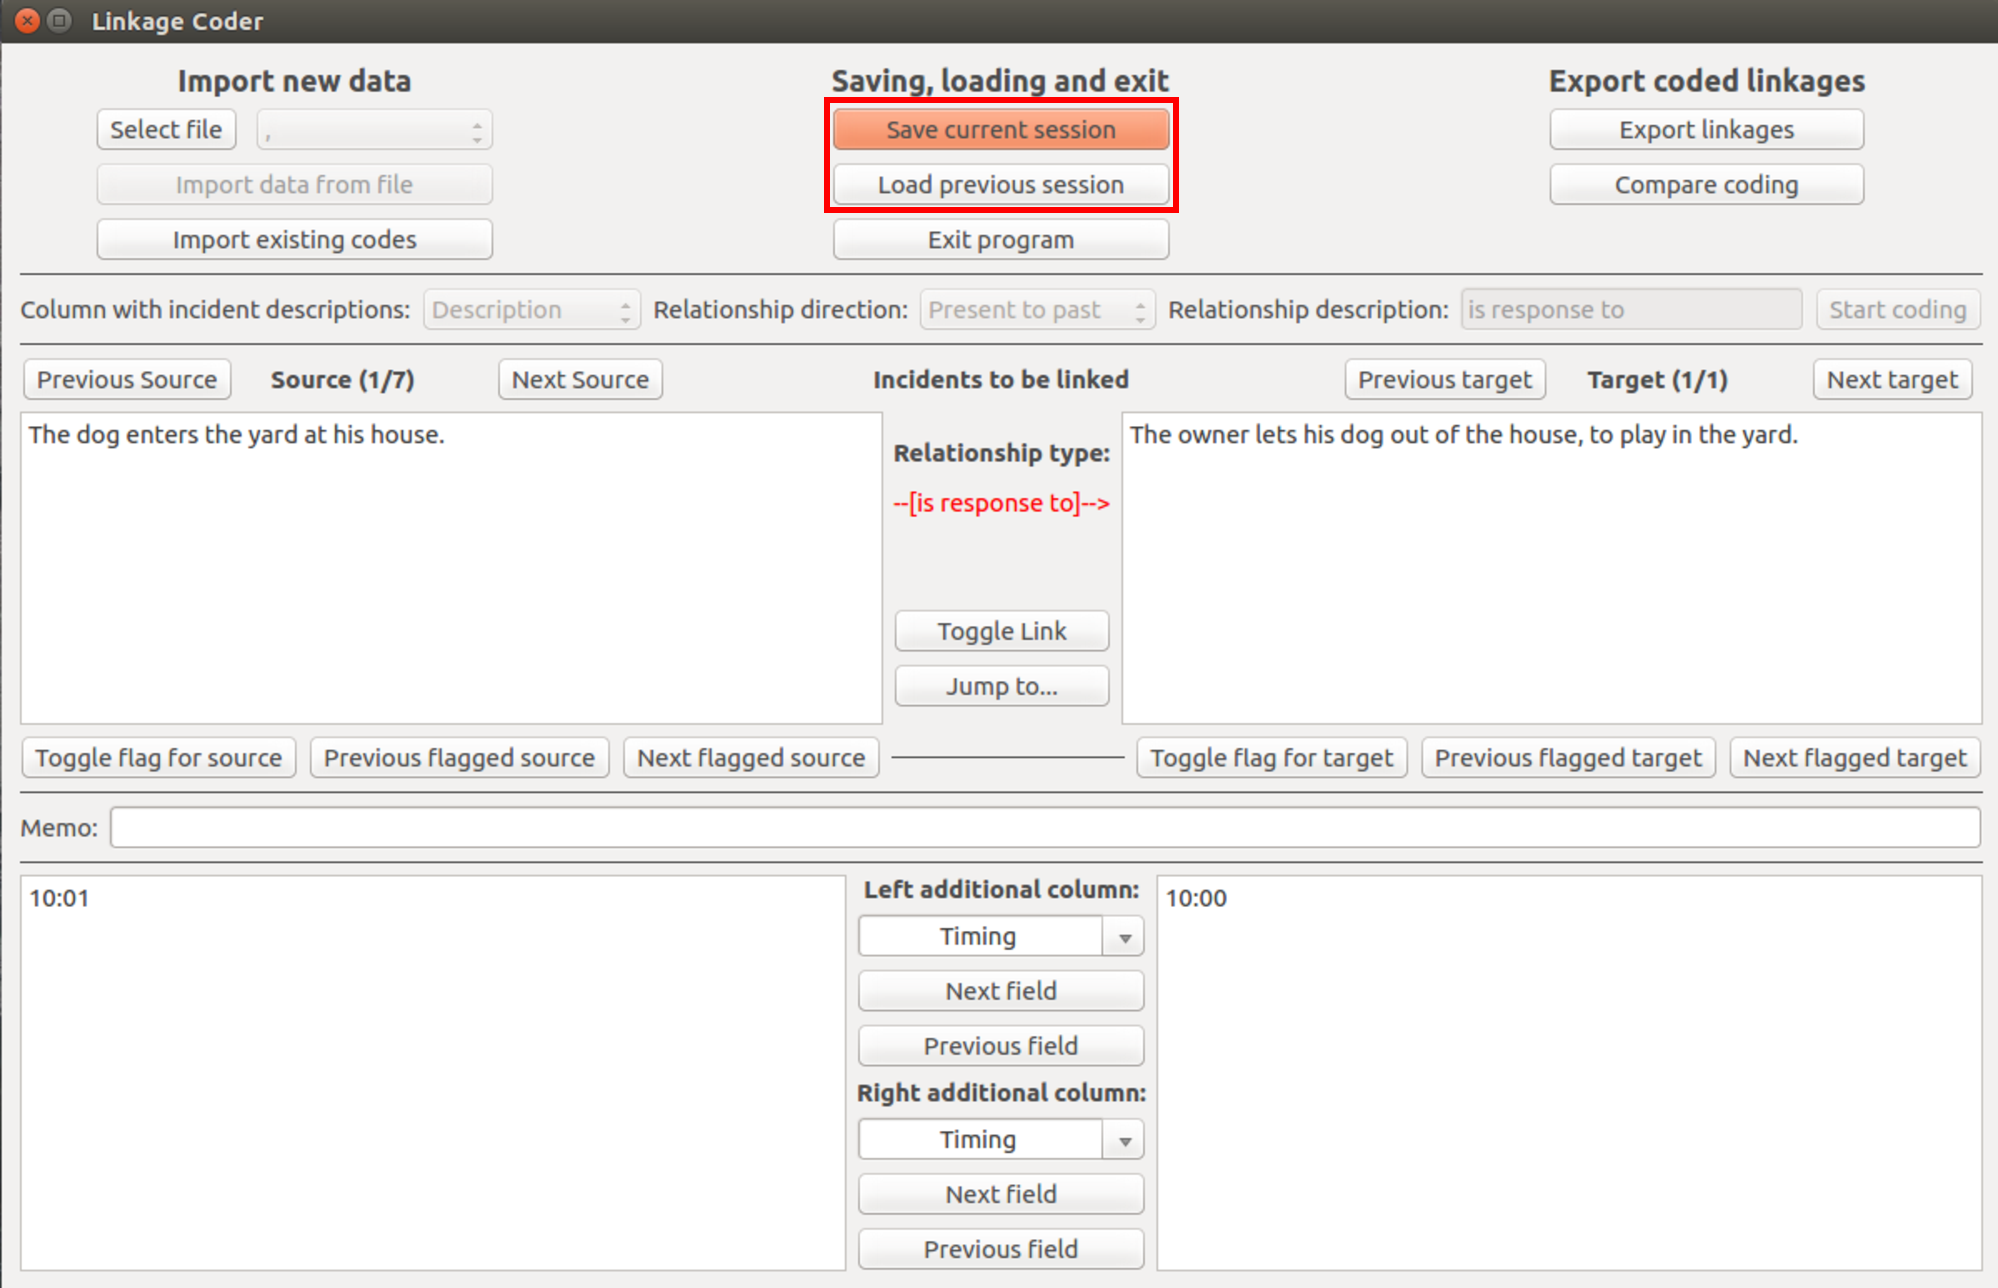
\includegraphics[width=100mm]{Screenshot_2.pdf}
%   \label{fig:saveload}
% \end{figure}

\section{Importing existing codes}
\label{sec:importingcodes}

Coding data is typically an iterative process, and it is possible that, during the coding process, the user makes changes to the data set being coded, for example, by adding new rows of data, by adding new columns of data, or by changing the contents of data cells. The program therefore allows the user to import existing codes from an old version of a given data set into a new version of the same data set. 

% \begin{figure}[h!]
%   \centering
%   \caption{Importing codes.}
%   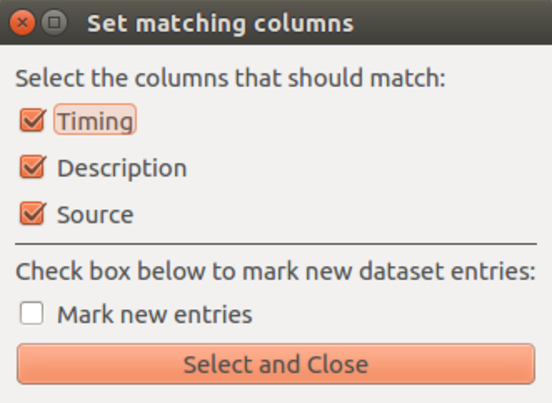
\includegraphics[width=40mm]{Screenshot_3.pdf}
%   \label{fig:importcodesfig}
% \end{figure}

The procedure for importing codes involves the following steps:
\begin{enumerate}
\item{The user should first make sure that the codes assigned to the \textbf{old version} of the data set are stored, by using the \textbf{Save session option} (see section \ref{sec:savingloadingdata}). At a later step, we will import the codes from this save file. For this example, we refer to this file as \textbf{Saved\textunderscore Codes.sav}.}
\item{After saving the codes assigned to the \textbf{old version} of the data set, we can import the \textbf{new version} of the data set, using the procedure described in section \ref{sec:loadingnewdataset}. Thus, the steps taken here are the same as when you would start coding a completely new data set.}
%\item{After the \textbf{new version} of the dataset has been loaded, you should click the \textbf{Import codes} button (see figure \ref{fig:importcodesfig}). You will first be shown a warning dialog, just to make sure that you can double check what you are doing. If you select \textbf{Ok} in the warning dialog, you will be shown a file dialog. Use this dialog to find the file with your saved codes (\textbf{Saved\textunderscore Codes.sav} in this example). Select and open this file.}
%\item{A new dialog will appear, the specific contents of which will depend on the contents of your data sets. An example is shown in figure \ref{fig:importcodesfig}, but yours will probably look different. The dialog will show the columns that the \textbf{old version} of your data set and the \textbf{new version} of your data set have in common. The program uses these columns to match entries in the \textbf{old version} of the data set with entries in the \textbf{new version} of the data set. The program will look at the data in the selected columns of both files. If it finds a row of data in the \textbf{new version} of the data set and a row of data in the \textbf{old version} of the data set that have the exact same contents in the selected columns, then the program will decide that these rows of data are the same. The program will then ensure that all the codes that are somehow associated with the row of data in the \textbf{old version} of the data set, are also associated with the corresponding row of data in the \textbf{new version} of the data set. By default, the program will inspect all columns, but you may want to deselect one or more columns if you decided to make small updates to the contents of these columns. However, for the codes to be imported correctly, the rows of data in both data sets need to be unique. For example, if you set the program to match the data sets using only one column, which has the same contents in multiple rows in one or both of the data sets, then the program will not be able to decide which codes are associated with which row of data. \textbf{In this case the codes will be assigned to the new data set erroneously, without warning!\footnote{In a later version of the program I will attempt to prevent this from happening altogether.} It is therefore very important that you always select a combination of columns that allows the program to identify each row of data individually.} If you just added some incidents to your data set, removed  incidents from your data set, and/or changed a few existing incidents, then it is usually safest to just have the program match the data sets using all columns. Otherwise, it should enough to select the column that indicates the timing of the incident, and the column that describes what happened in that incident, because having two incidents with the exact same timing, and the exact same contents (description) would probably never make sense, because they would describe the same activity, making one of them redundant. I advise you to always as many columns as possible to prevent problems like this from occurring. See figure \ref{fig:importingcodesdiagram} for a schematic overview that may help to understand the process.}
\item{You also have the option to have the program mark any new entries in the \textbf{new version} of the data set. This means that, while checking the columns you have selected, the program will also remember any rows of data in the \textbf{new version} of the data set that it could not match to any rows of data in the \textbf{old version} of the data set. These entries will be marked (see \ref{sec:markingincidents}), so that you can easily find them while coding the data.}
\item{If you happened to have changed data in one of the rows of the data set, that is, the row was already present in the \textbf{old version} of the data set, but you changed some of the contents of that row of data in the \textbf{new version} of the data set (in one of the selected columns), that row of data will be treated as new entry, and any codes assigned to that entry will be lost.}
\item{The program should now return to the main screen, and any attribute codes and relationship codes that were present in the save file that you loaded should now also be available in the current session. Moreover, any incidents that already had codes assigned to them in that save file should now also have those codes assigned to them in the current session.}
\end{enumerate}

\begin{figure}[h!]
  \centering
  \caption{Schematic overview of matching of data set entries.}
  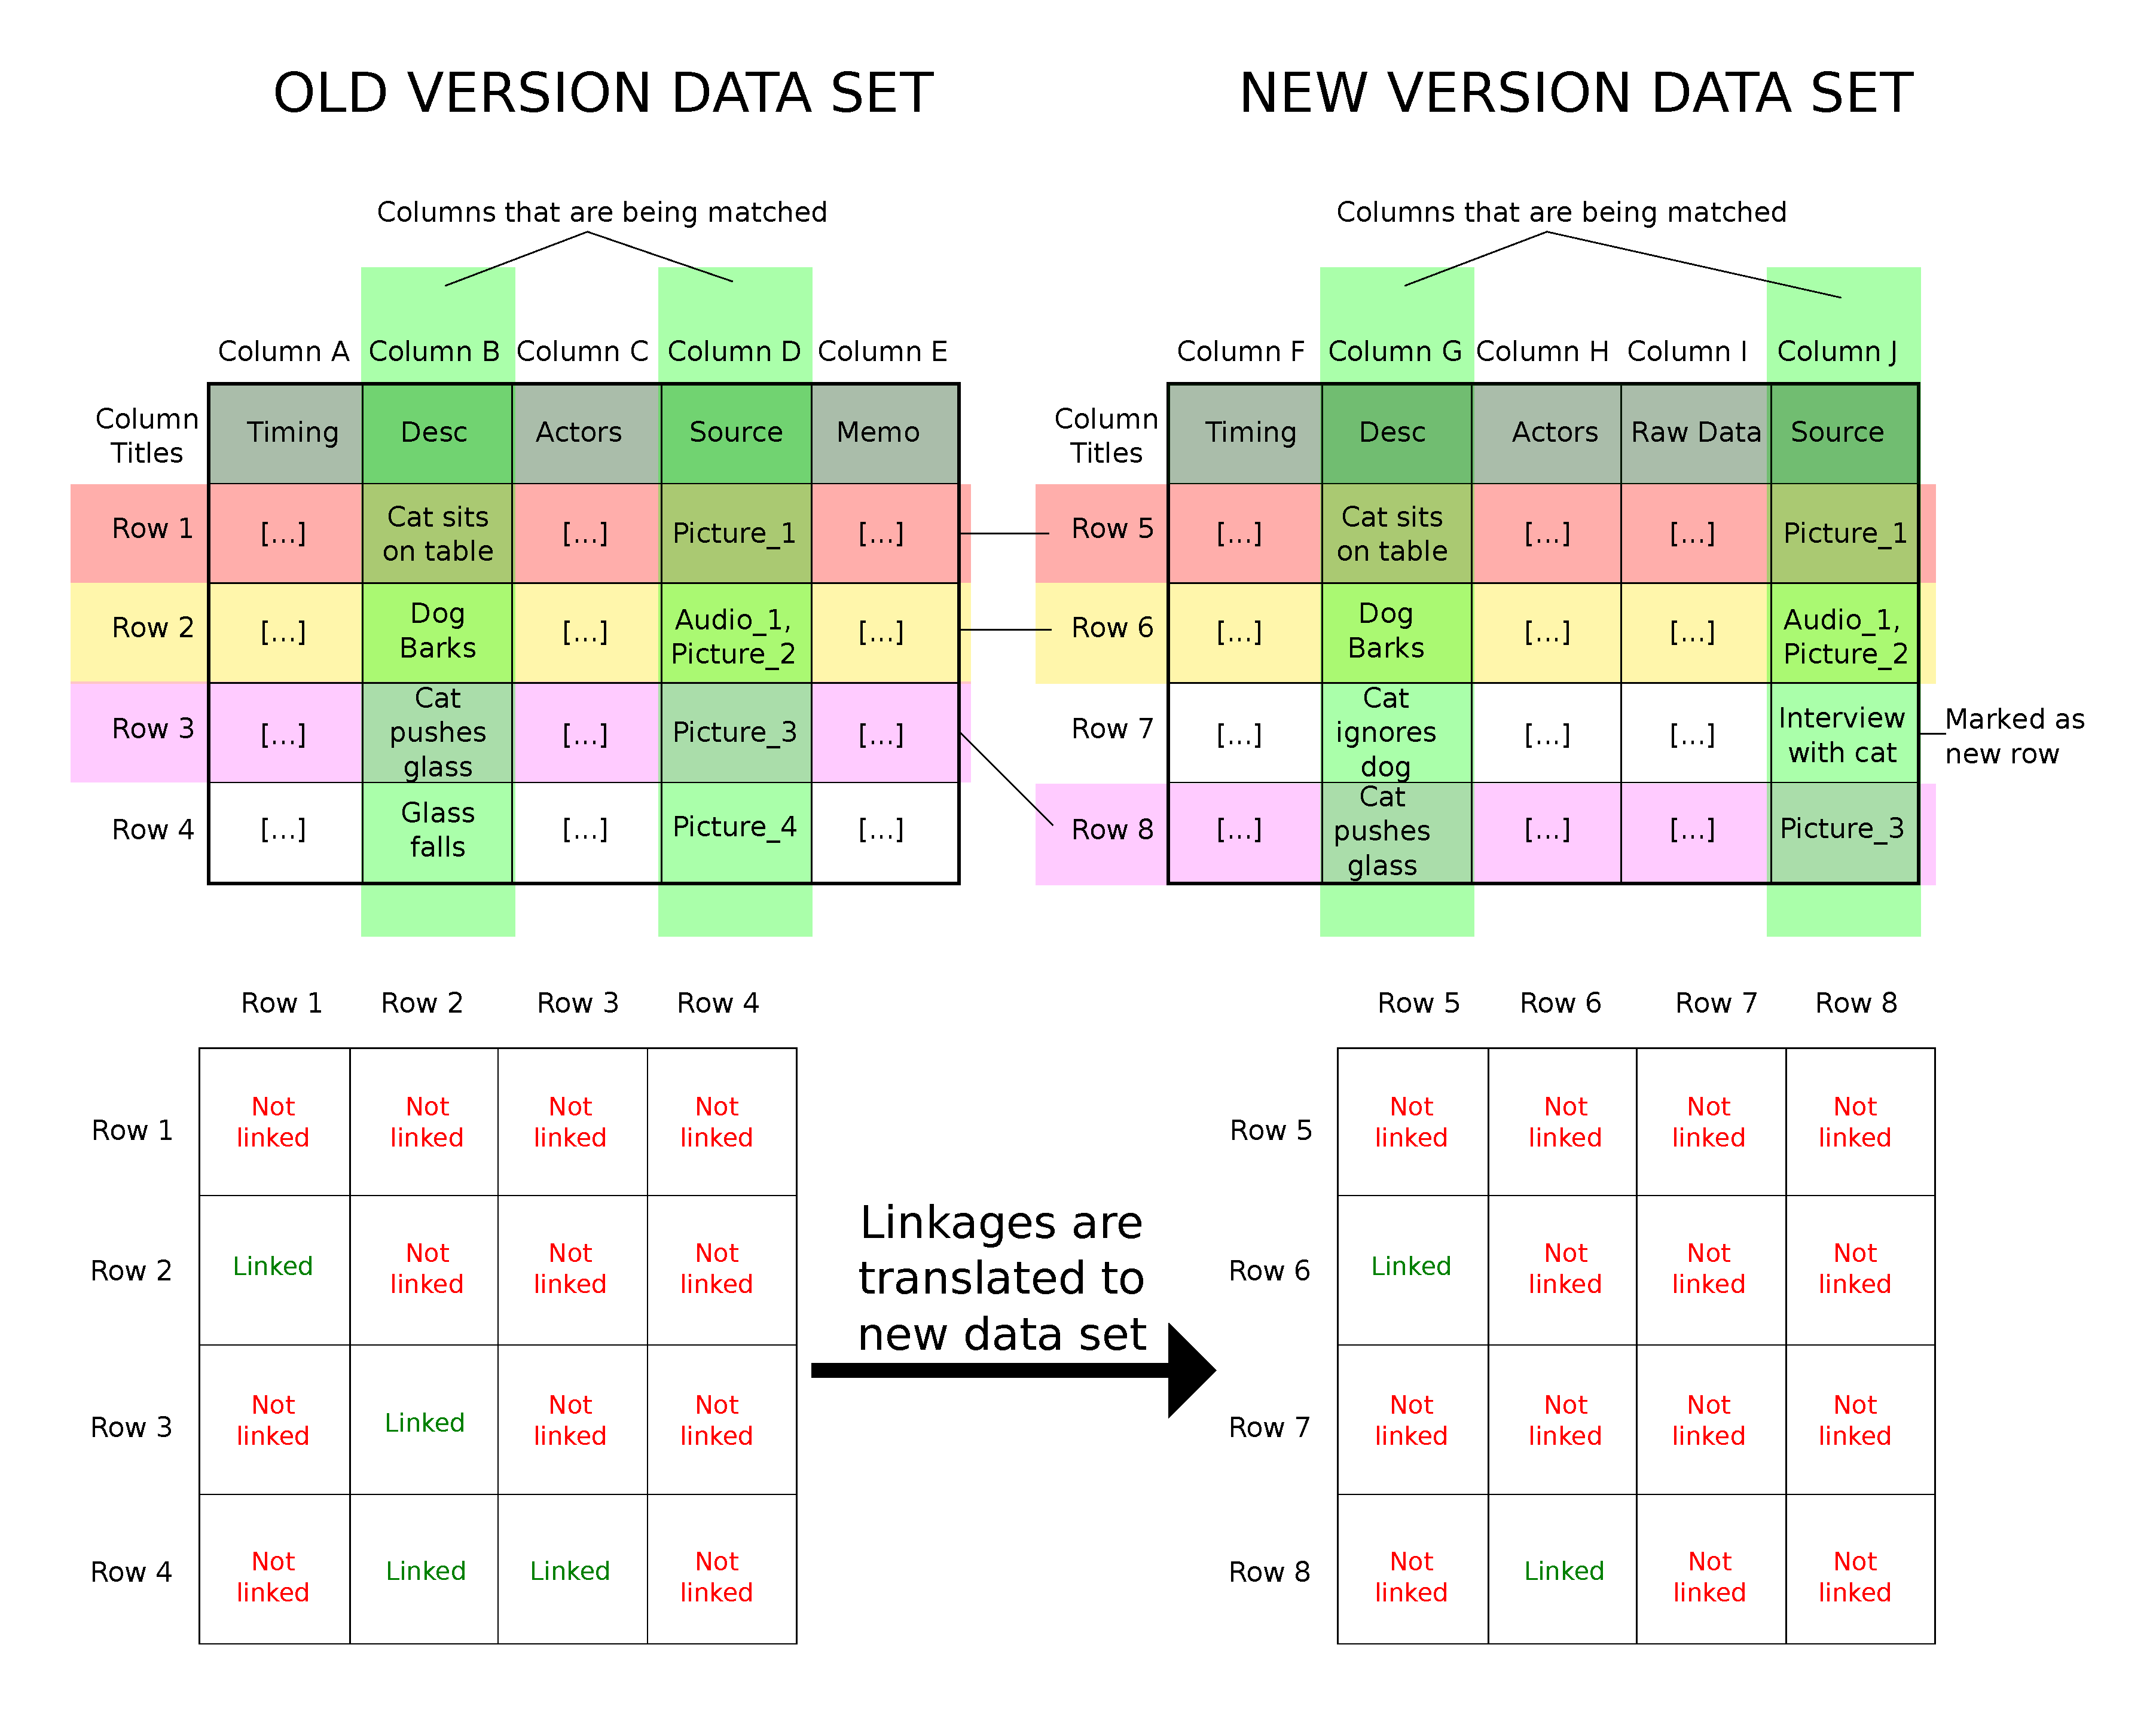
\includegraphics[width=100mm]{Diagram_1.pdf}
  \label{fig:importingcodesdiagram}
\end{figure}

\subsection{Problems when importing codes}
\label{sec:problemsimportingcodes}

There are several things that could go wrong when importing codes from an old data set into a new one. One problem would occur if you do not select any columns to be imported in the appropriate dialog. In this case the program will simply report that no columns were selected, and it will take no further action. Another similar problem would occur if you try to import codes from a data set that has no columns in common with the data set that is loaded into your current session. In this case the dialog where columns can be selected will be empty (except for the option to mark new entries). If you try to proceed, the program will behave as if no columns were selected (see above), report an error, and take no further action.

Another problem may be that some of the codes assigned to entries in the \textbf{old version} of the data set do not get imported into the \textbf{new version} of the data set, even though these entries appear in both. This should only happen if something changed in the contents of these entries (and only in the contents of those columns that the program tries to match). Even if you made only small changes in the contents of the selected columns, the program will treat the corresponding entry as a new, uncoded entry. 

A more difficult problem will occur if you do not select columns that allow the program to identify each row of data in the \textbf{old version} and/or the \textbf{new version} of your data set individually (see the box below for an explanation).

\begin{framed}
  \textbf{Example to illustrate problem when importing non-unique rows}

  First, imagine that you select two columns (\(C_1\) and \(C_2\)), the contents of which need to be matched by the program. Second, imagine that in the \textbf{old version} of the data set, there exist two incidents (two rows in the data set; \(I^{old}_1\) and \(I^{old}_2\)) that have identical data in those columns. In addition, imagine that the sets of codes (\(S_1\) and \(S_2\)) that you assigned to these two incidents are different (\(S_1 \rightarrow I^{old}_1\) and \(S_2 \rightarrow I^{old}_2\)).

  When comparing the two versions of the data set, the program encounters one of these rows of data \(I^{old}_1\). If it also encounters a row of data in the \textbf{new version} of the data set that has the exact same data in \(C_1\) and \(C_2\) (let us call this row \(I^{new}_x\)), it will think it has found a match, and assign the corresponding codes to the corresponding entry in the \textbf{new version} of the data set (\(S_1 \rightarrow I^{old}_1\) becomes \(S_1 \rightarrow I^{new}_x\)). However, the program then proceeds, and it will also encounter the other row of data \(I^{old}_2\), the contents of which (in columns \(C_1\) and \(C_2\)) also match with those of \(I^{new}_x\). As a result, the program will simply overwrite the codes that already existed (\(S_1 \rightarrow I^{new}_x\) gets overwritten by \(S_2 \rightarrow I^{new}_x\)). More importantly, the program will not recognise that something has gone wrong, so it will do this work silently, without reporting any error (also see figure \ref{fig:overwritingcodes}).
\end{framed}

\begin{figure}[h!]
  \centering
  \caption{Codes that are silently overwritten due to multiple matches.}
  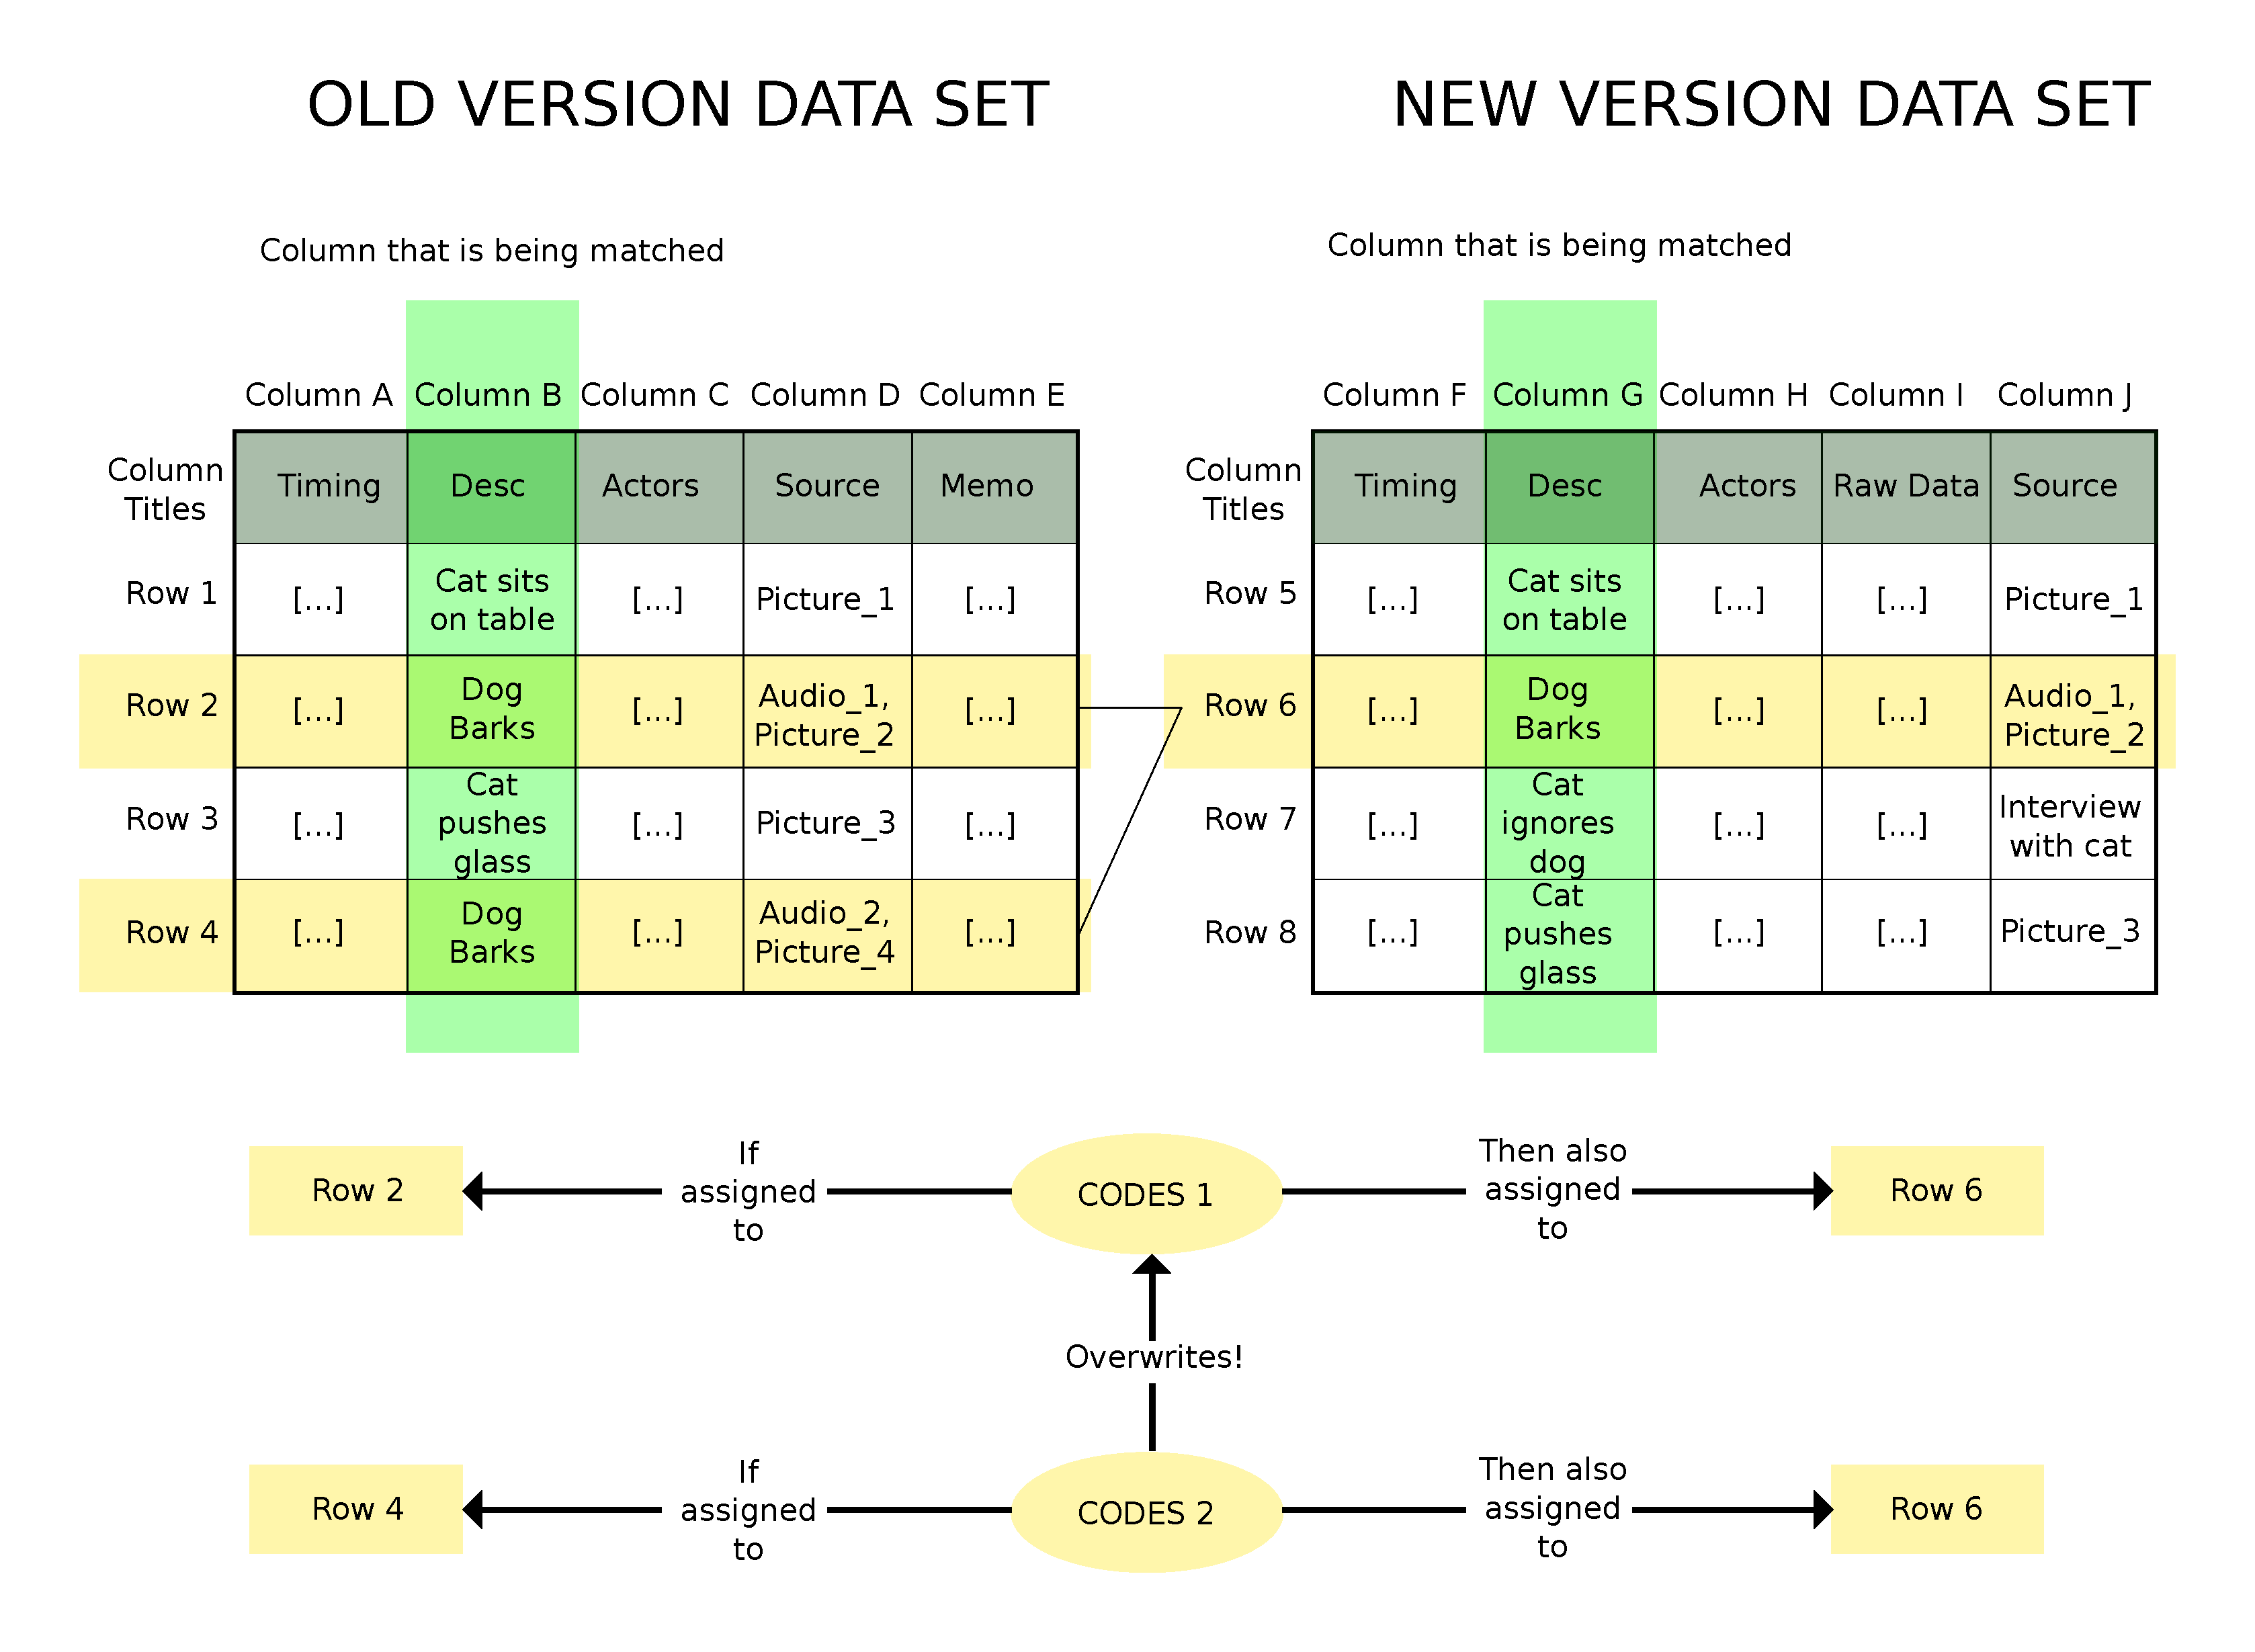
\includegraphics[width=100mm]{Diagram_2.pdf}
  \label{fig:overwritingcodes}
\end{figure}

To prevent this problem from occurring, you must always make sure that, based on the columns that you selected in the import dialog, the program will never find two rows of data that are exactly the same. As explained in section \ref{sec:importingcodes}, it should typically be enough to select (1) a column that indicates the timing of the incident, and (2) a column that contains the qualitative description of the incident itself (see section \ref{sec:datasets} for the assumptions that the program makes about how your data set is structured). It is unlikely that two incidents have the exact same contents in these two columns (because then they would simply refer to the exact same incident).

\section{Navigating through the data}
\label{sec:navigatingdata}

The program, to some extent, enforces a specific way to walk through your data set. As explained in section \ref{sec:datasets}, the program assumes that your data are chronologically ordered, with the incidents that occurred earliest at the top, and the incidents that occurred latest at the bottom. When you start coding a new data set, the program will always assume that you wish to start the coding process with the earliest incident. The program will present to you one incident at a time, showing you details on the currently selected incident in up to two fields (see figure %\ref{fig:incidentsoverview}). 

% \begin{figure}[h!]
%   \centering
%   \caption{Overview of incident navigation section.}
%   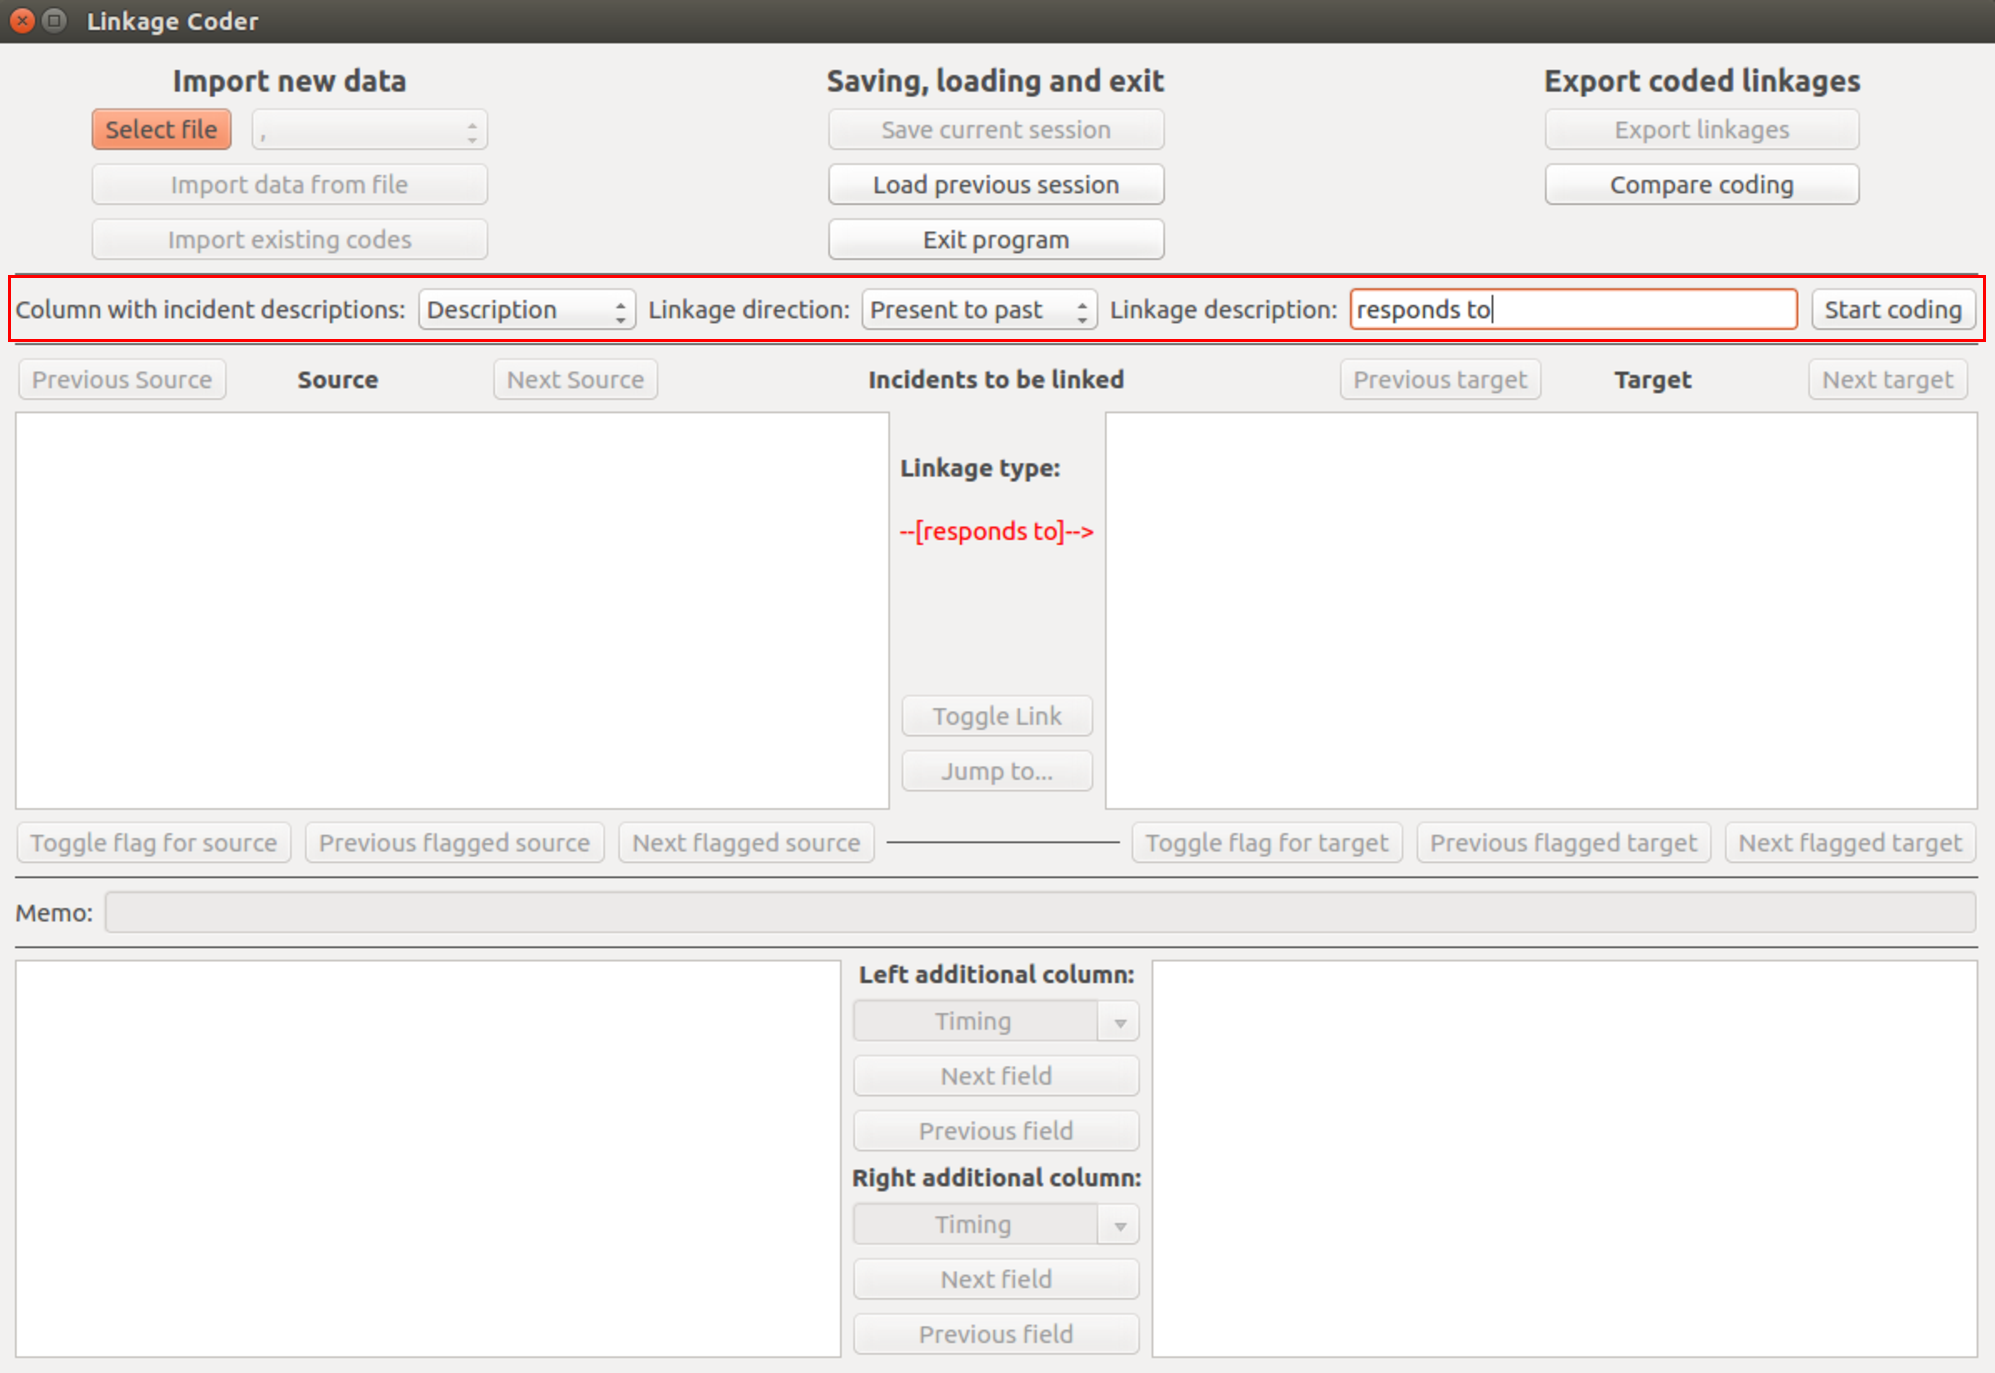
\includegraphics[width=100mm]{Screenshot_4.pdf}
%   \label{fig:incidentsoverview}
% \end{figure}

In the two fields, the program can display the contents of any of the columns of your original data set. Below each field, you will find buttons that you can use to choose which column of the original data set to display in the field (the first column of data is selected by default for both fields). The arrow buttons will go to the previous or next column, and the drop-down menu can be used to simply jump to a specific column. 

Typically, you will want to assign codes to the incidents based on the information provided in one or more columns of data, such as the description of the activity that the incident captures, and possibly the raw text (from the sources of data) on which this description is based. The program can show up to two columns of data, which, in my own experience, is a nice balance between having a good overview, and not having to process too much information at a time.

Typically, you will create new codes on the fly (see chapter \ref{chap:usingtheprogram2}), assign appropriate codes to the current incident, and then move on to the next incident. Above the fields with the information on the current incident, you will see an indicator of which incident is currently selected (``\textbf{Incident ([current]/[total])}''). To navigate the incidents, use the buttons above the text fields (see figure %\ref{fig:incidentsoverview}). These buttons are pretty straightforward. The \textbf{Previous incident} button navigates to the previous incident in the data set. If the currently selected incident is the first in the data set, clicking this button will let you jump to the last incident in the data set. The \textbf{Next incident} button lets you navigate to the next incident in the data set. If the currently selected incident is the last incident in the data set, clicking this button will let you jump to the first incident in the data set.

You will also see a button called \textbf{Jump to}. Clicking this button will open a small dialog that allows you to type the index number of the incident that you want to jump to. If you type an 'illegal' number (e.g., a number below 1, or a number that exceeds that total number of incidents in the data set) nothing will happen. 

\subsection{Marking incidents}
\label{sec:markingincidents}

In the area demarcated in figure %\ref{fig:incidentsoverview}, you will also find three buttons that refer to flagged incidents (\textbf{Previous flagged incident}, \textbf{Next flagged incident}, and \textbf{Toggle flag}). Flags can be used to mark incidents that you would like to return to later. If you click the \textbf{Toggle flag} button, an exclamation mark will appear next to the index to show that this incident is currently flagged %(see figure \ref{fig:flaggedincident}).

% \begin{figure}[h!]
%   \centering
%   \caption{Indication of flagged incident.}
%   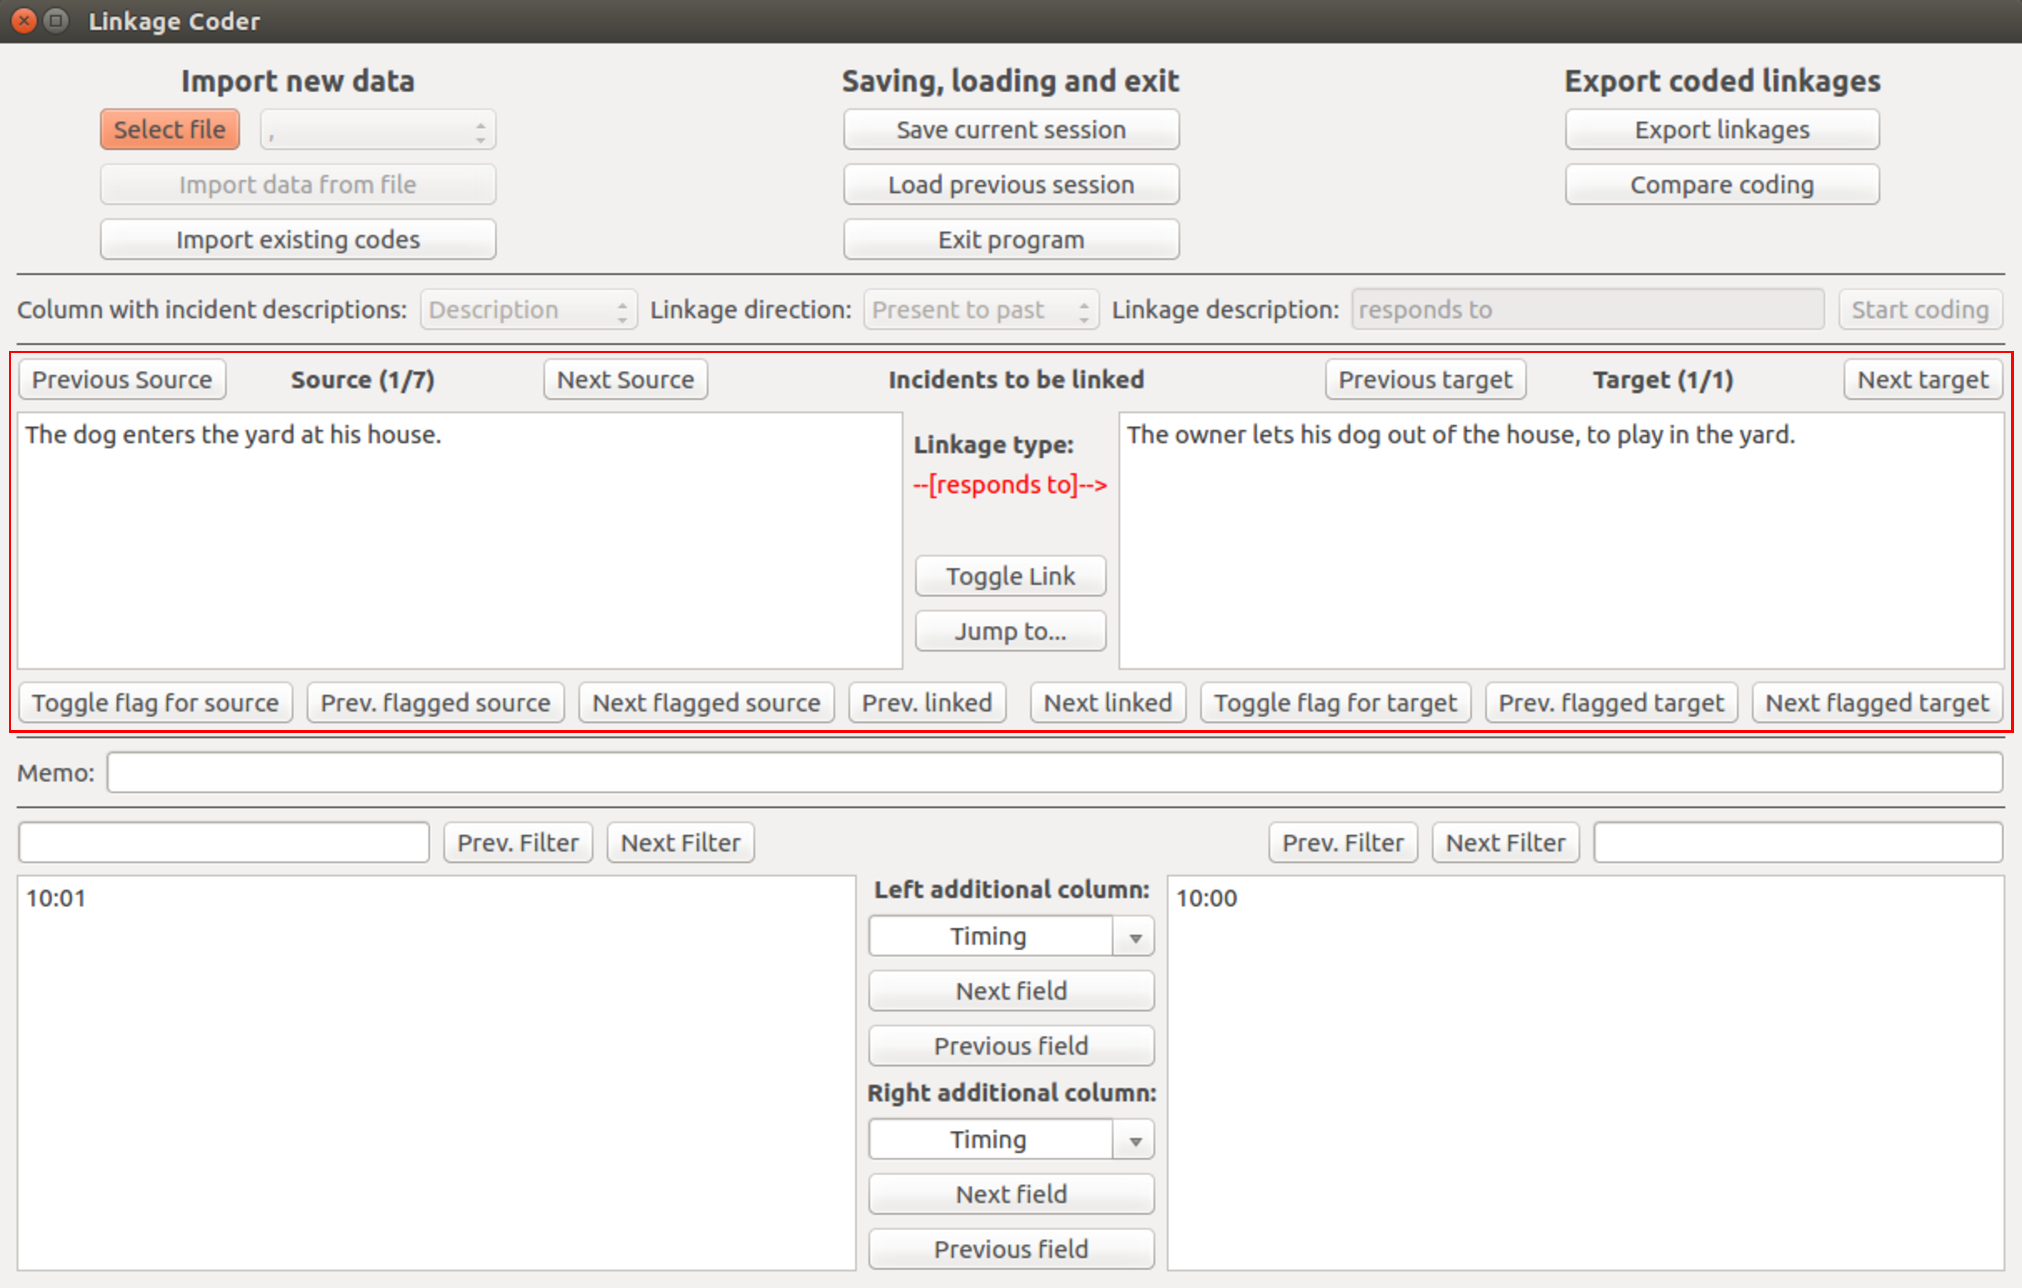
\includegraphics[width=40mm]{Screenshot_5.pdf}
%   \label{fig:flaggedincident}
% \end{figure}

If you later want to return to your flagged incident, you can use the \textbf{Previous flagged incident} or the \textbf{Next flagged incident} button. These buttons work similar to the \textbf{Previous incident} and the \textbf{Next incident} buttons, but they will skip all incidents that are not flagged. This should allow you to relatively easily find incidents that you flagged earlier.

\begin{framed}
\textbf{Automatically flagging new incidents when importing codes}
  
  As described in section \ref{sec:importingcodes}, when you import codes from a previously stored session into a new version of a data set, you will also have the option to mark any new incidents. This means that the program will automatically flag all incidents that are in the \textbf{new version} of the data set that you are currently coding, but that were not in the \textbf{old version} of the data set from which you are importing the codes. This allows you to always easily find the incidents that have not received any codes before. 
\end{framed}

\section{Exporting data}
\label{sec:exportingdata}

In chapter \ref{chap:usingtheprogram2} I explain in depth how the coding program itself works. Once you have coded a data set, and you want to export the results, you can click the \textbf{Open export dialog} button. This will open a new dialog, where you can select several export options (see figure %\ref{fig:exportdialog}).

% \begin{figure}[h!]
%   \centering
%   \caption{The export dialog.}
%   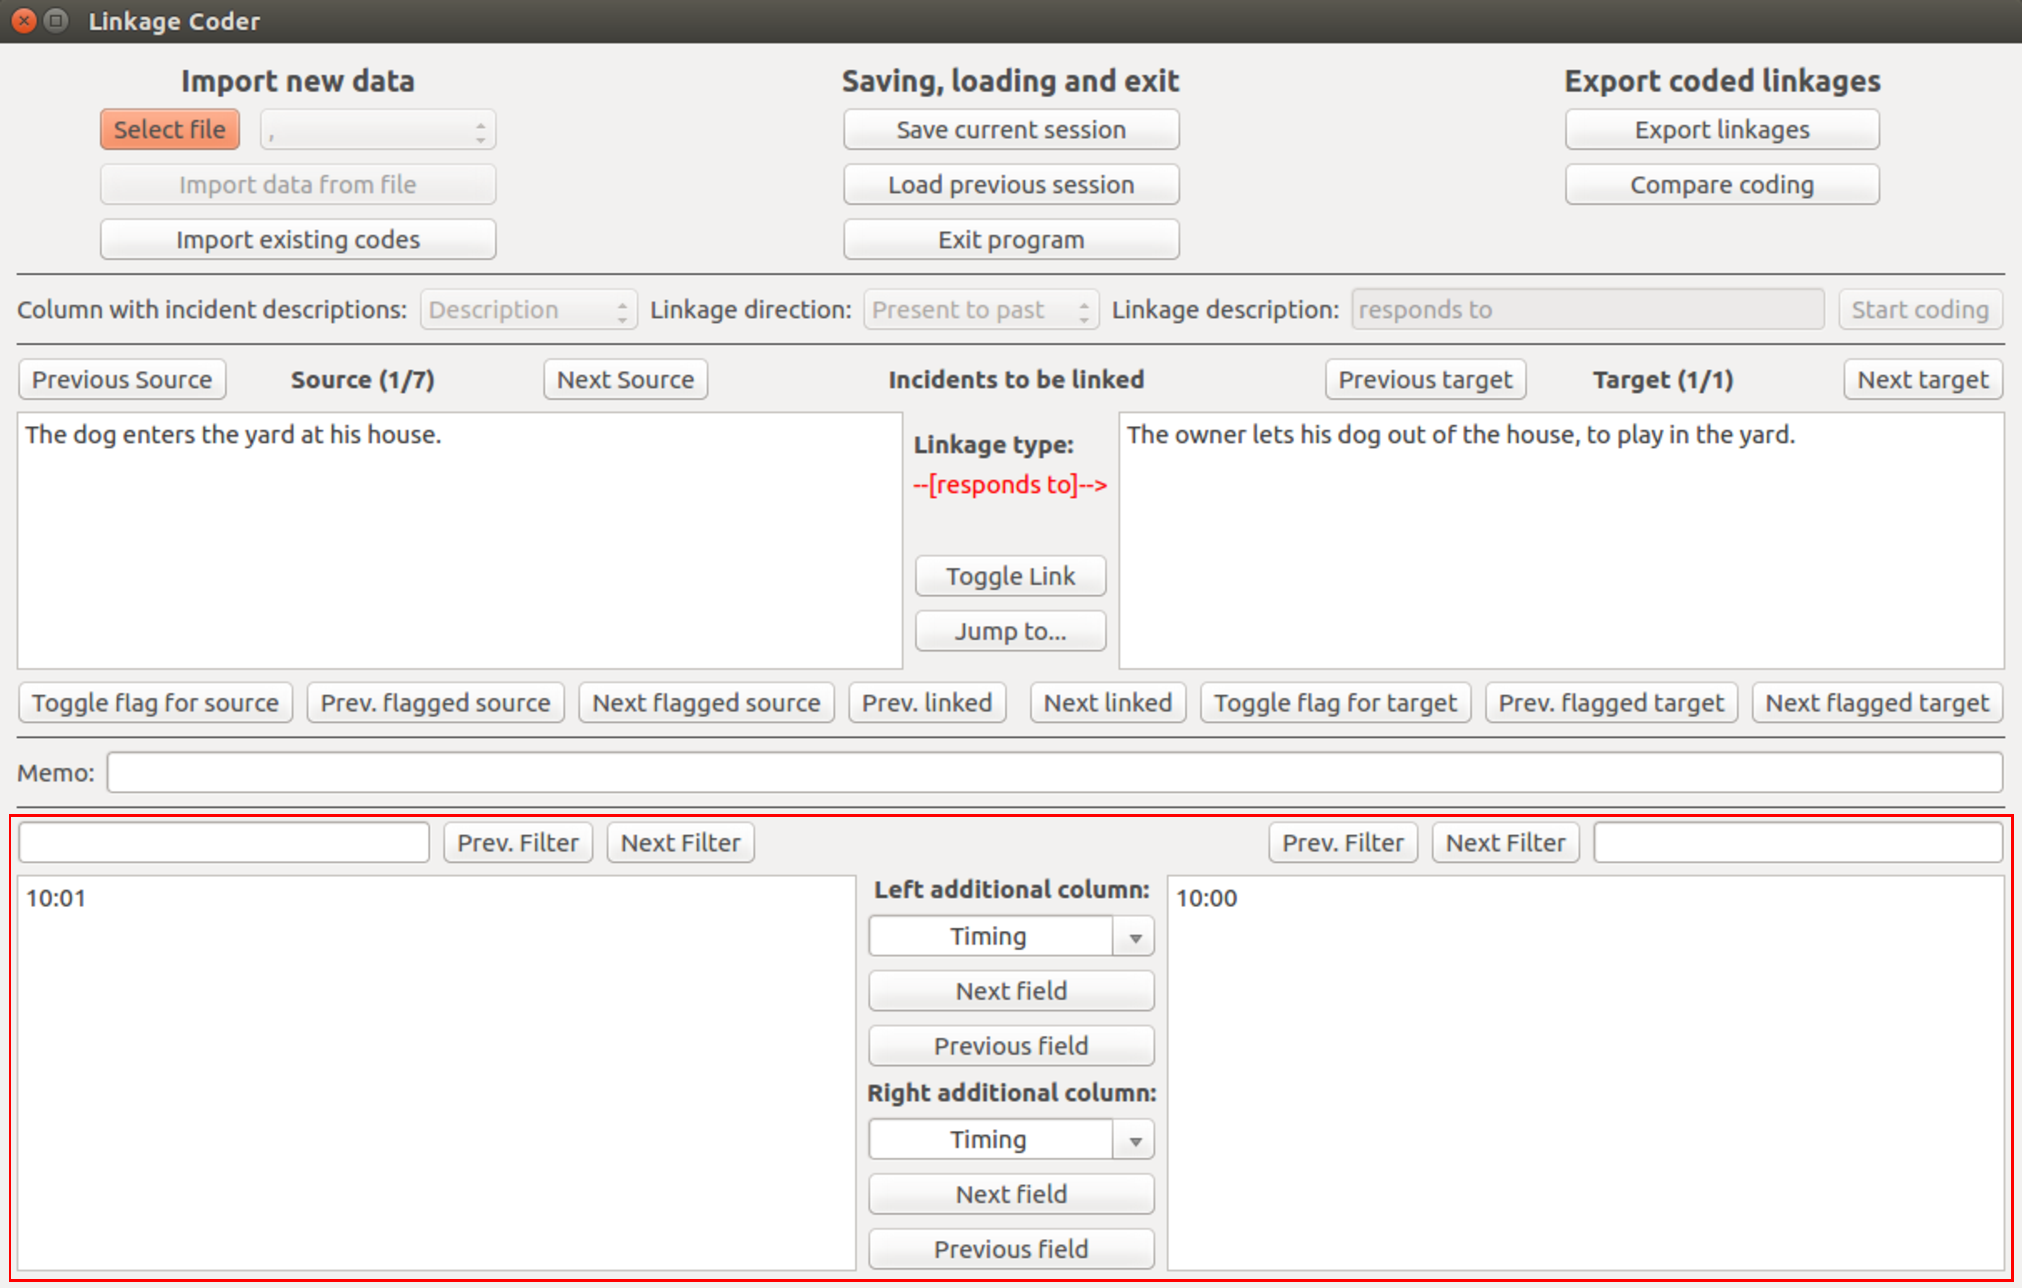
\includegraphics[width=40mm]{Screenshot_6.pdf}
%   \label{fig:exportdialog}
% \end{figure}

The first set of options, under the header \textbf{Incident export options}, allows you to assign properties to your incidents. These properties are simply the contents of the various columns of the data set that you imported. In fact, if you select all the properties, using the corresponding tick boxes, one of the files exported will simply be a near-identical copy of the original data set that you imported, the only difference being that every incident will be assigned a unique ID, numbered from 1 to \(N\), where \(N\) is the total number of incidents in your data set. These incidents, and any properties that you select for them, will be written to a file that is called \textbf{``Incidents\textunderscore Nodes.csv''}. As the name of the file suggests, this is a node list, which in this case is structured such that it can be immediately imported into Gephi, my favourite network visualisation program\footnote{See https://gephi.org. I offer no instructions on how to import data into Gephi here. Various guides for that are available elsewhere. Indeed, the data can also be imported into other software, although you might have to make small changes for that to work.}. 

By default, the program will also export (1) all attributes that you have assigned to incidents, (2) all categories that you have assigned to incident attributes, (3) all relationships that you have assigned to incidents, (4) all attributes that you have assigned to entities in relationships, and (5) all categories that you have assigned to entity attributes. You can deselect any of these options, although categories can only be exported if their corresponding attributes are also exported, and entity attributes and categories can only be exported if you also export relationships. Depending on what options you select, the following will be exported:

To understand more about what you could possibly do with all these files, please read chapter \ref{chap:whatisnext}.


\section{Log files and exiting the program}
\label{sec:logfilesandexiting}

It will probably come as no surprise to you that the default way to close the program is to click the \textbf{Exit program} button. Alternatively, you could close the dialog of the program in the same way you would close any dialog in your OS.

Just before the program closes, it will export a log file to the \textbf{"logs/"} folder that is located in the folder from which you run the program (if this folder does not exist yet, the program will create it). The log file will be time stamped with the date and time at which it was created. In the log file, you will find a lot of details of various operations that you have performed while using the program, such as navigating to other incidents, assigning or unassigning attributes and/or relationships to incidents, and several other things. These logs are created silently and automatically.

The logs are designed to help you make the coding process more transparent. For example, they may help you retrace your steps if at some point in the coding process you run into some kind of problem, and do not remember how you got there. The log also records which columns of your data set you were inspecting when assigning certain attributes or relationships, helping you to remember on what information you based your decision to assign these codes. I do not expect that anyone will be terribly interested to ever inspect these log files, but it may be reassuring to know that they are there if you need them.  


\chapter{Using the program: Coding features}
\label{chap:usingtheprogram2}

\section{Introduction to coding}
\label{sec:introductiontocoding}


\chapter{What is next?}
\label{chap:whatisnext}



\section{Graph databases}
\label{sec:graphdatabases}

At the time of writing this manual, I am experimenting with the use of graph databases, which are, in very simple terms, databases in which all data are either stored as \textbf{nodes}, as \textbf{relationships between nodes}, or as \textbf{properties} of nodes or relationships. For me, storing data this way is ideal, because I usually like to present event data in some ``networked form'', and with graph databases there are very few steps required between storing data and presenting data in such a form. As discussed in section \ref{sec:partofbiggerprogram}, I intend to integrate the \textbf{\emph{Event Coder}} program in a bigger program at some point. My intention is for this bigger program to interface directly with a graph database, without the user ever having to worry about how this works. For now, however, the user will need to use third-party solutions for creating such a graph database, and import the coded data into such a database manually.

The graph database technology that I currently work with myself is the Neo4j Community Edition\footnote{See \url{https://neo4j.com/}.}, because (1) it is open source, which is something that I encourage, and (2) because it uses a query language and interface that I find very useful\footnote{I also see important drawbacks to Neo4j. In my opinion the configuration of Neo4j on your system, and the creation and management of new databases could have been made more intuitive. If you are completely new to Neo4j, it might take a while for you to get a solid grasp of how it works.}. I will not go into the details of how to use Neo4j here, because that would take me well beyond the scope of this manual. There is a wealth of information that can be found on the website of Neo4j\footnote{See, for example, \url{https://neo4j.com/docs/}.}, as well as on numerous other online forums. One of the files exported by the \emph{\textbf{Event Coder}} program (\textbf{"CYPHER.txt"} is a list of Cypher commands (Cypher is the language used by Neo4j) that the user can simply copy and paste into the Neo4j interface to recreate the complete, coded data set as a Neo4j database.    

Figure %\ref{fig:graphdatabaseexample} shows a screenshot of a Neo4j database that I created in this way, using some made-up data that I also used throughout the manual. In this screenshot, the larger red nodes represent incidents, the larger green nodes, represent relationships indicated by these incidents, the pink nodes represent entities in these relationships, the yellow nodes are attributes that have been assigned to incidents or entities, and so on. All information that we created when coding the data is represented in this graph as a node, a relationship, or a property of a node or relationship.

% \begin{figure}[h!]
%   \centering
%   \caption{A coded version of our fictional data set stored in a graph database.}
%   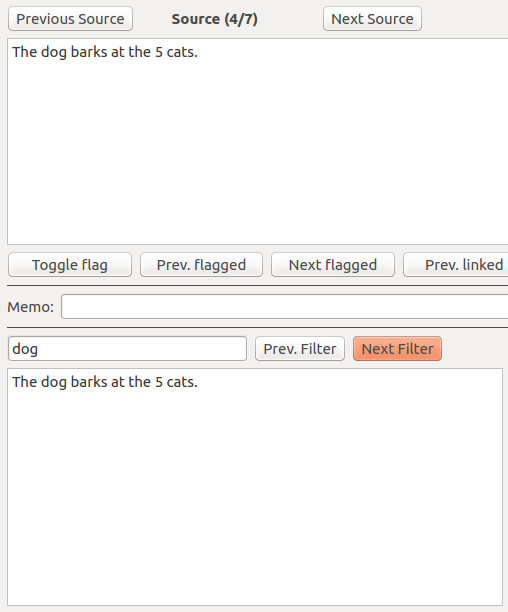
\includegraphics[width=100mm]{Screenshot_23.pdf}
%   \label{fig:graphdatabaseexample}
% \end{figure}

There are many other possibilities with the Cypher query language. This does not actually tell you anything that you could do with these data in terms of analysis, but I hope it does make clear that it offers a lot of flexibility in how you store, present, and structure your data. Once you manage to put your data into a graph structure, it is easy to convert your data in the various forms required by different software packages.

\section{Creating event graphs}
\label{sec:creatingeventgraphs}

Another program that I have recently created is the \emph{\textbf{Linkage Coder}} program. This program imports the exact same type of data sets as the \emph{\textbf{Event Coder}} program, but its purpose is different: Rather than being a tool for qualifying incidents (with attributes and relationships), the \textbf{\emph{Linkage Coder}} program can be used to identify relationships \emph{between} incidents. For example, certain activities in a given data set may have occurred \emph{in response to} other activities in that data set. The \emph{\textbf{Linkage Coder}} program is designed to identify such linkages between activities and make them explicit (through qualitative coding).

The \textbf{\emph{Event Coder}} program and the \textbf{\emph{Linkage Coder}} program are intimately related. In fact, I plan to integrate both of them in a larger program in the future (see section \ref{sec:partofbiggerprogram}). I use the joint output of the programs to create \emph{event graphs}. These are graphs in which the nodes represent events, and the edges represent relationships between events\footnote{For an example of a publication in which event graphs are used, see Spekkink, W. A. H., \& Boons, F. A. A. (2016). The Emergence of Collaborations. \emph{Journal of Public Administration Research and Theory}, 26(4), 613–630.}. The \textbf{\emph{Linkage Coder}} program helps me to create the basic structure of event graphs, and the \textbf{\emph{Event Coder}} program helps me to qualify the events, for example, by identifying what types of activities these events represent.

%Figure \ref{fig:eventgraph} shows a visualisation of an event graph that I recently used in a presentation. In this graph, the events are laid out from left to right based on the time of their occurrence. The colours represent different types of activities (something we could identify with the \emph{\textbf{Event Coder}} program), and the edges represent which activities occurred in response to which other activities (something we could identify with the \textbf{\emph{Linkage Coder}} program).

% \begin{figure}[h!]
%   \centering
%   \caption{Example of event graph.}
%   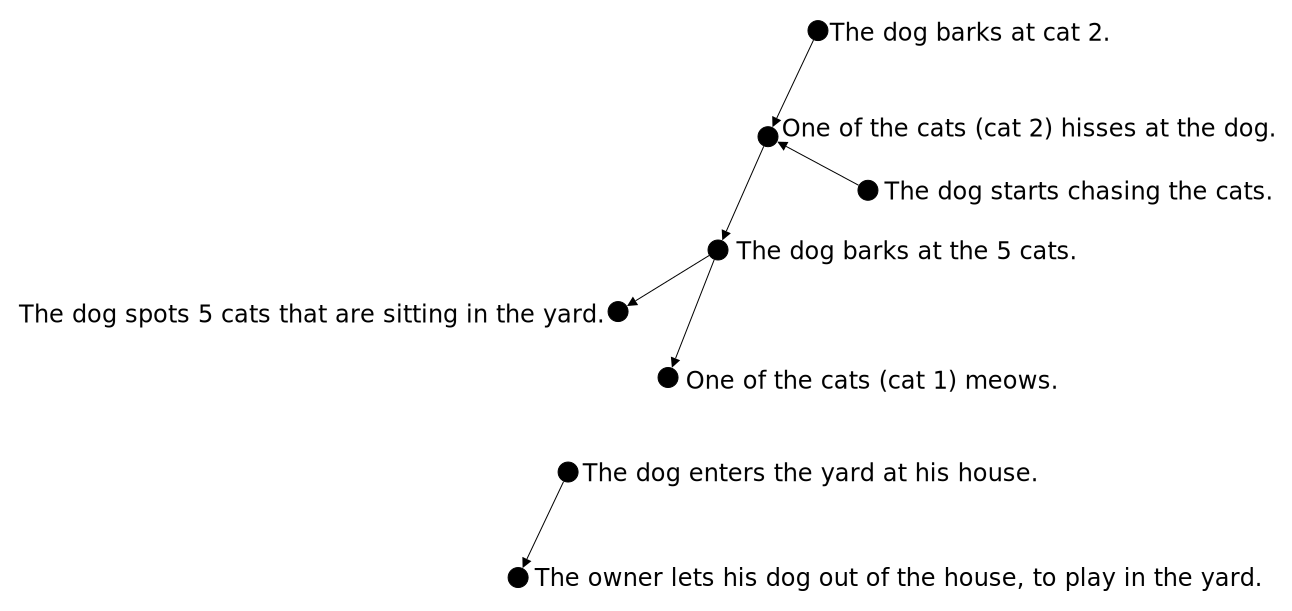
\includegraphics[width=80mm]{Diagram_6.png}
%   \label{fig:eventgraph}
% \end{figure}


\chapter{Contact details}
\label{chap:contactdetails}

At the time of writing this manual, I work as a Research Associate at the Sustainable Consumption Institute (SCI) of the University of Manchester.

Wouter Spekkink \\
The Sustainable Consumption Institute \\
The University of Manchester \\
188 Waterloo Place, Oxford Road \\
M13 9PL, Manchester \\
The United Kingdom

Email address (office): \href{mailto:wouter.spekkink@manchester.ac.uk}{wouter.spekkink@manchester.ac.uk} \\
Email address (personal): \href{mailto:wouterspekkink@gmail.com}{wouterspekkink@gmail.com}

Website: \url{http://www.wouterspekkink.org} \\
Github page (where I upload source code): \url{https://github.com/WouterSpekkink}





\end{document}